\documentclass[aspectratio=169]{beamer}
\usepackage{will_handley_beamer}
\usepackage{title_page}
\usetikzlibrary{positioning}
\usetikzlibrary{calc}
\usetikzlibrary{fit}

% Commands
% --------
% - \arxiv{arxiv number}
% - \cols{width}{lh column}{rh column}
% -  \begin{fig(left|right)}[fractional width (e.g 0.6) ]{name of image}
%        content of other column
%    \end{fig(left|right)}

% Talk details
% ------------
\title{Next generation inference tools for cosmology and beyond}
%\subtitle{}
\date{23\textsuperscript{rd} Jan 2024}

\begin{document}

\begin{frame}
    \titlepage
\end{frame}

\begin{frame}
    \frametitle{The golden age of cosmology data}
    \begin{columns}
        \column{0.45\textwidth}
        \begin{itemize}
            \item Over our research lifetimes we will see next-generation data rates across the electromagnetic spectrum \& beyond:
                \begin{description}
                    \item[Radio] SKA \textit{et al}
                    \item[Micro] SO/CMB-S4
                    \item[IR] JWST, Roman (WFIRST)
                    \item[Optical] Euclid, DESI, Rubin (LSST), EELT
                    \item[X-ray] Athena
                    \item[Gamma-ray] e-ASTROGAM
                    \item[Gravitational] LIGO/Virgo/Kagra + LISA
                    \item[Particle] CTA, IceCube, KM3NeT
                \end{description}
        \end{itemize}
        \column{0.55\textwidth}

        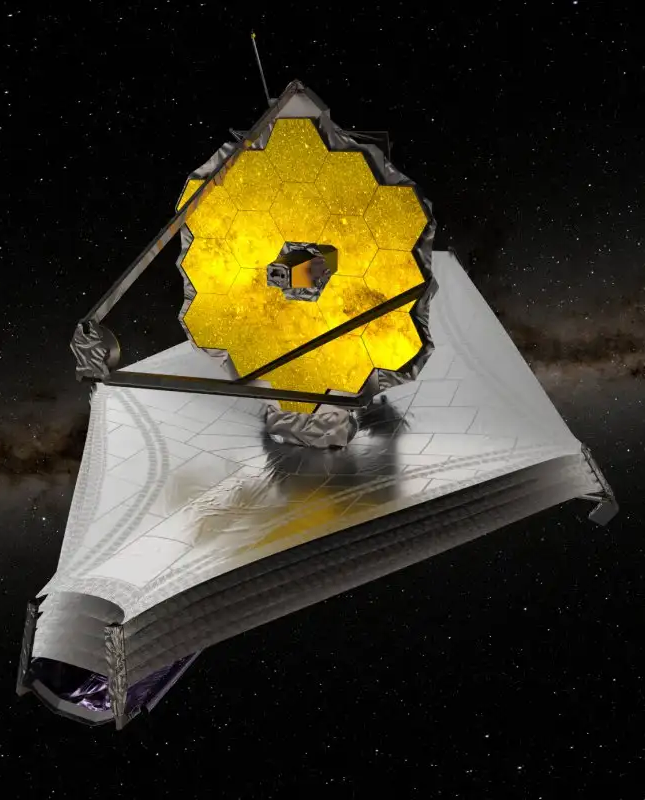
\includegraphics[height=0.145\textwidth]{figures/telescopes/jwst}%
        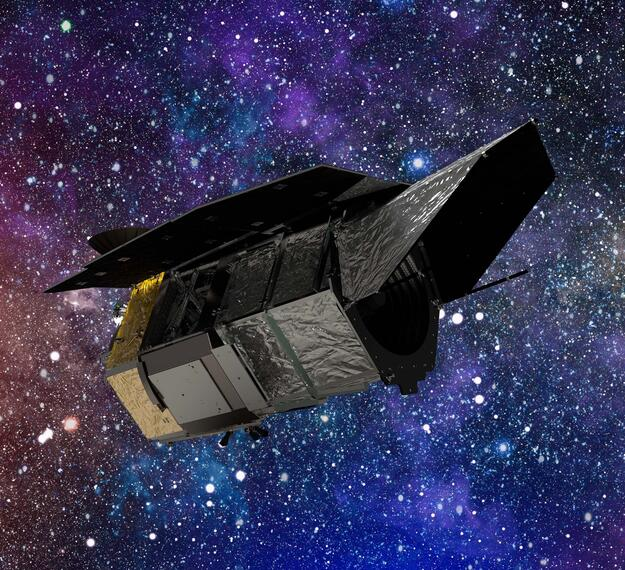
\includegraphics[height=0.145\textwidth]{figures/telescopes/roman}%
        \includegraphics[height=0.145\textwidth]{figures/telescopes/euclid}%
        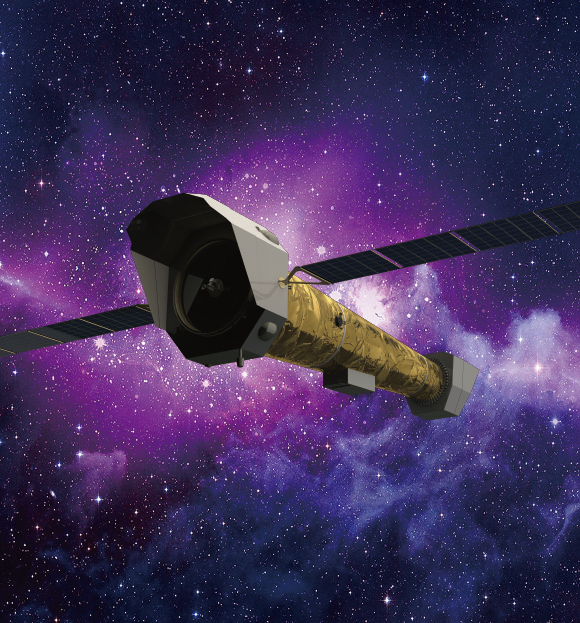
\includegraphics[height=0.145\textwidth]{figures/telescopes/athena}%
        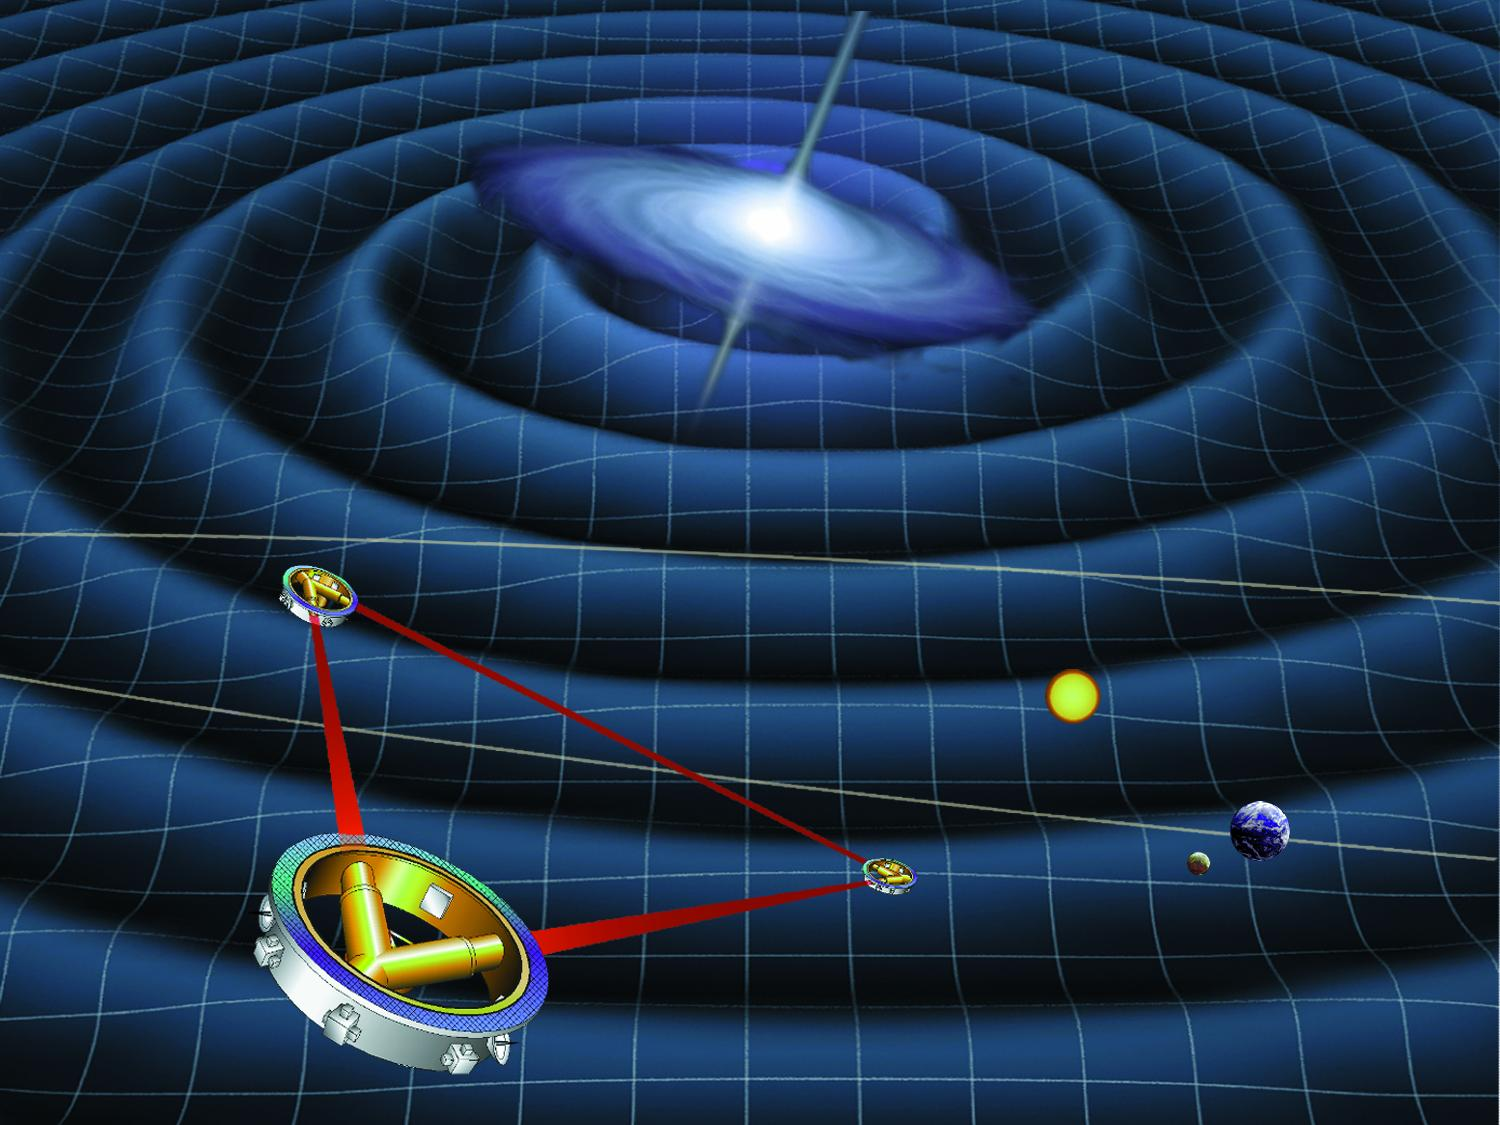
\includegraphics[height=0.145\textwidth]{figures/telescopes/lisa}%
        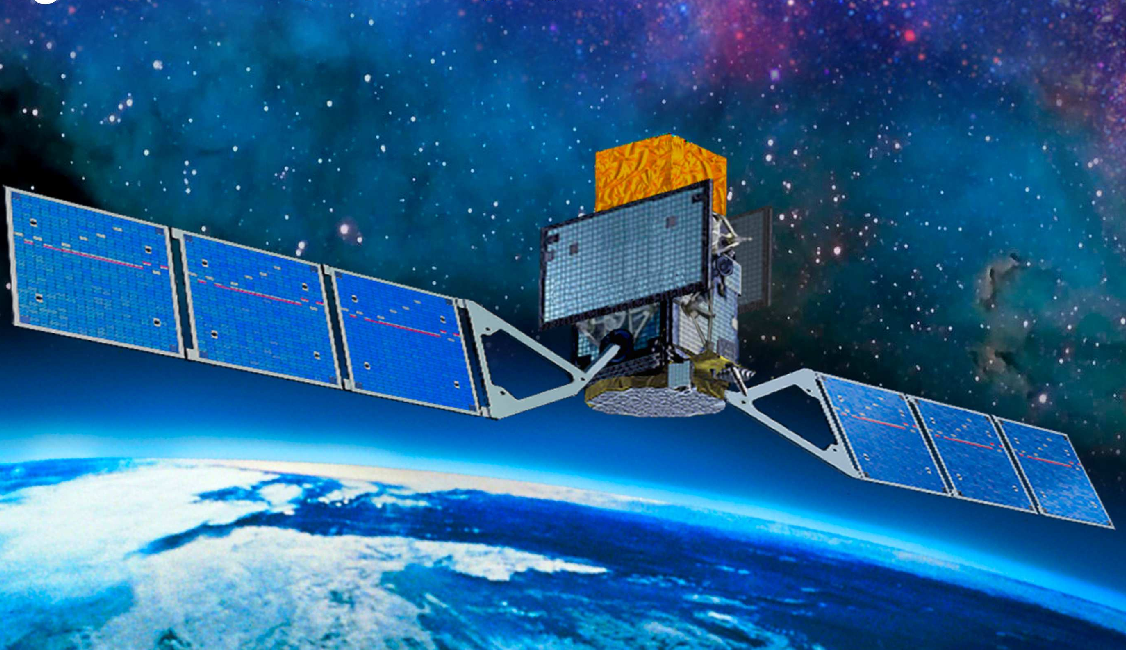
\includegraphics[height=0.145\textwidth]{figures/telescopes/e-ASTROGAM}%
        \vspace{-1pt}

        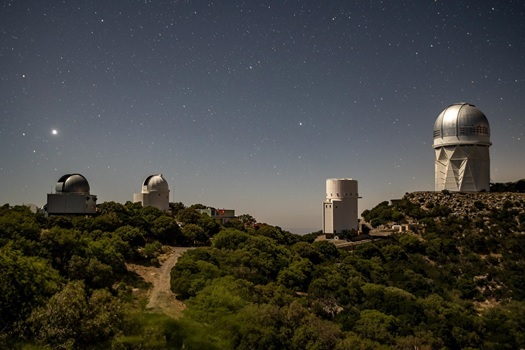
\includegraphics[height=0.15183\textwidth]{figures/telescopes/desi}%
        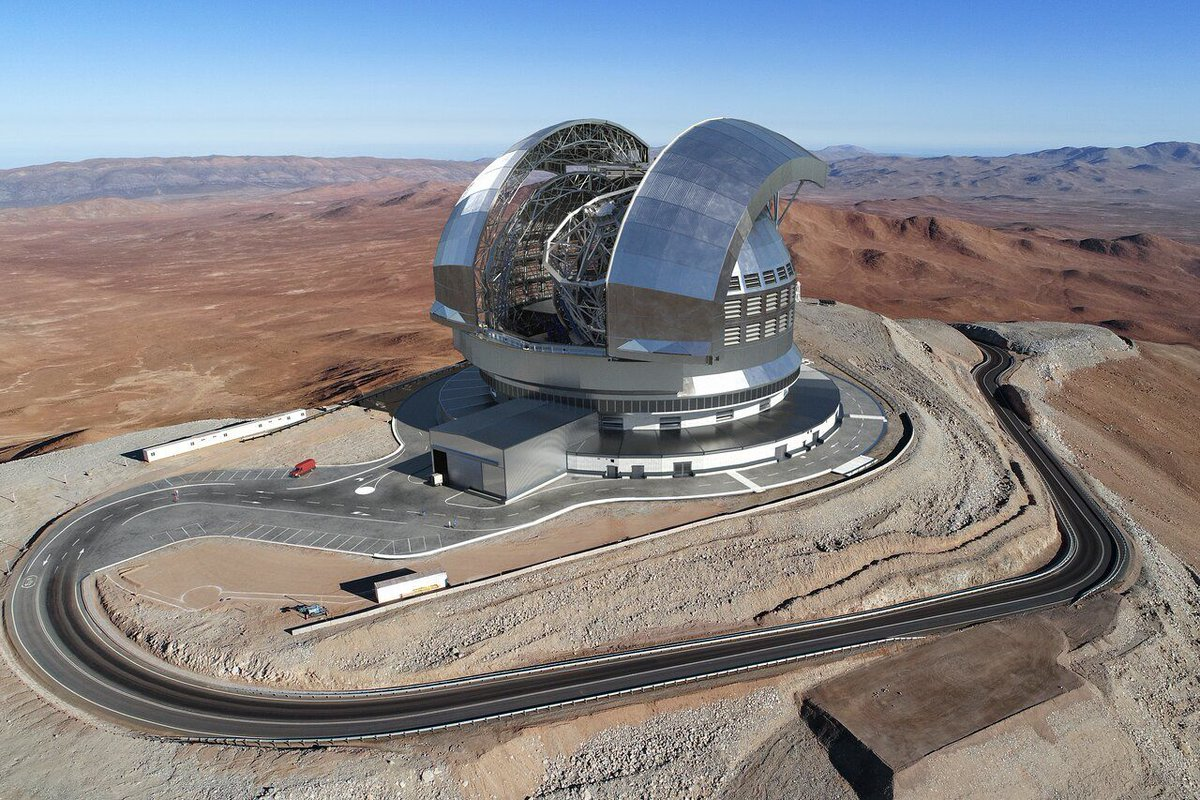
\includegraphics[height=0.15183\textwidth]{figures/telescopes/eelt}%
        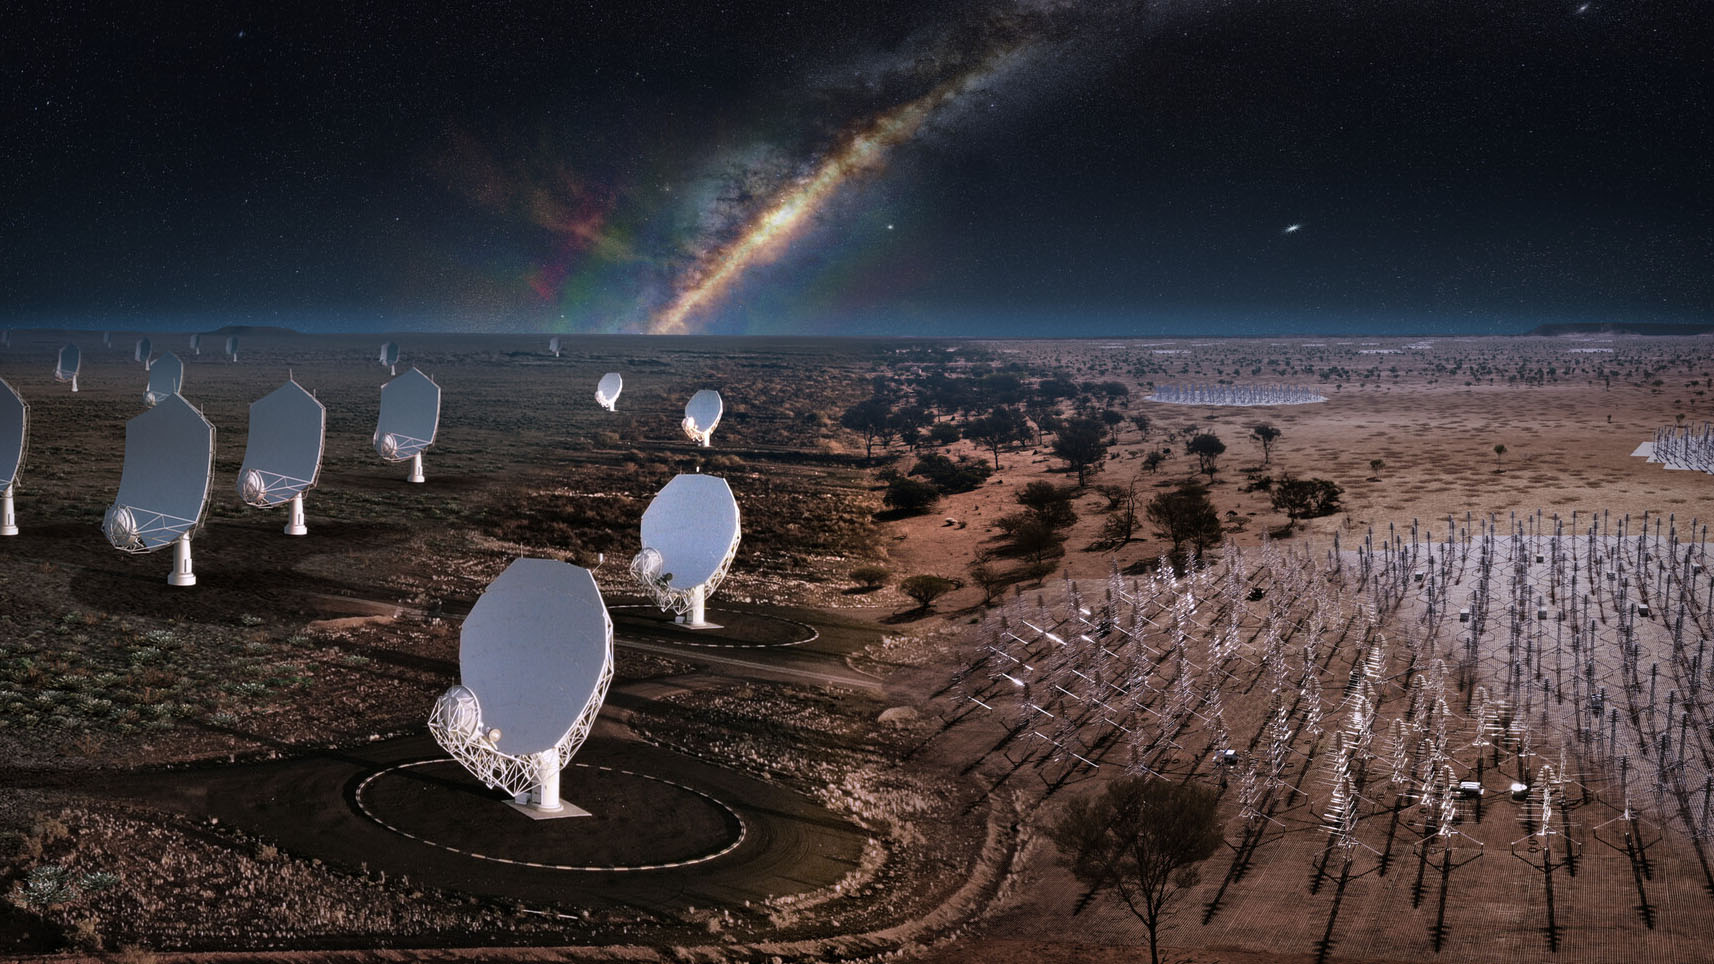
\includegraphics[height=0.15183\textwidth]{figures/telescopes/ska}%
        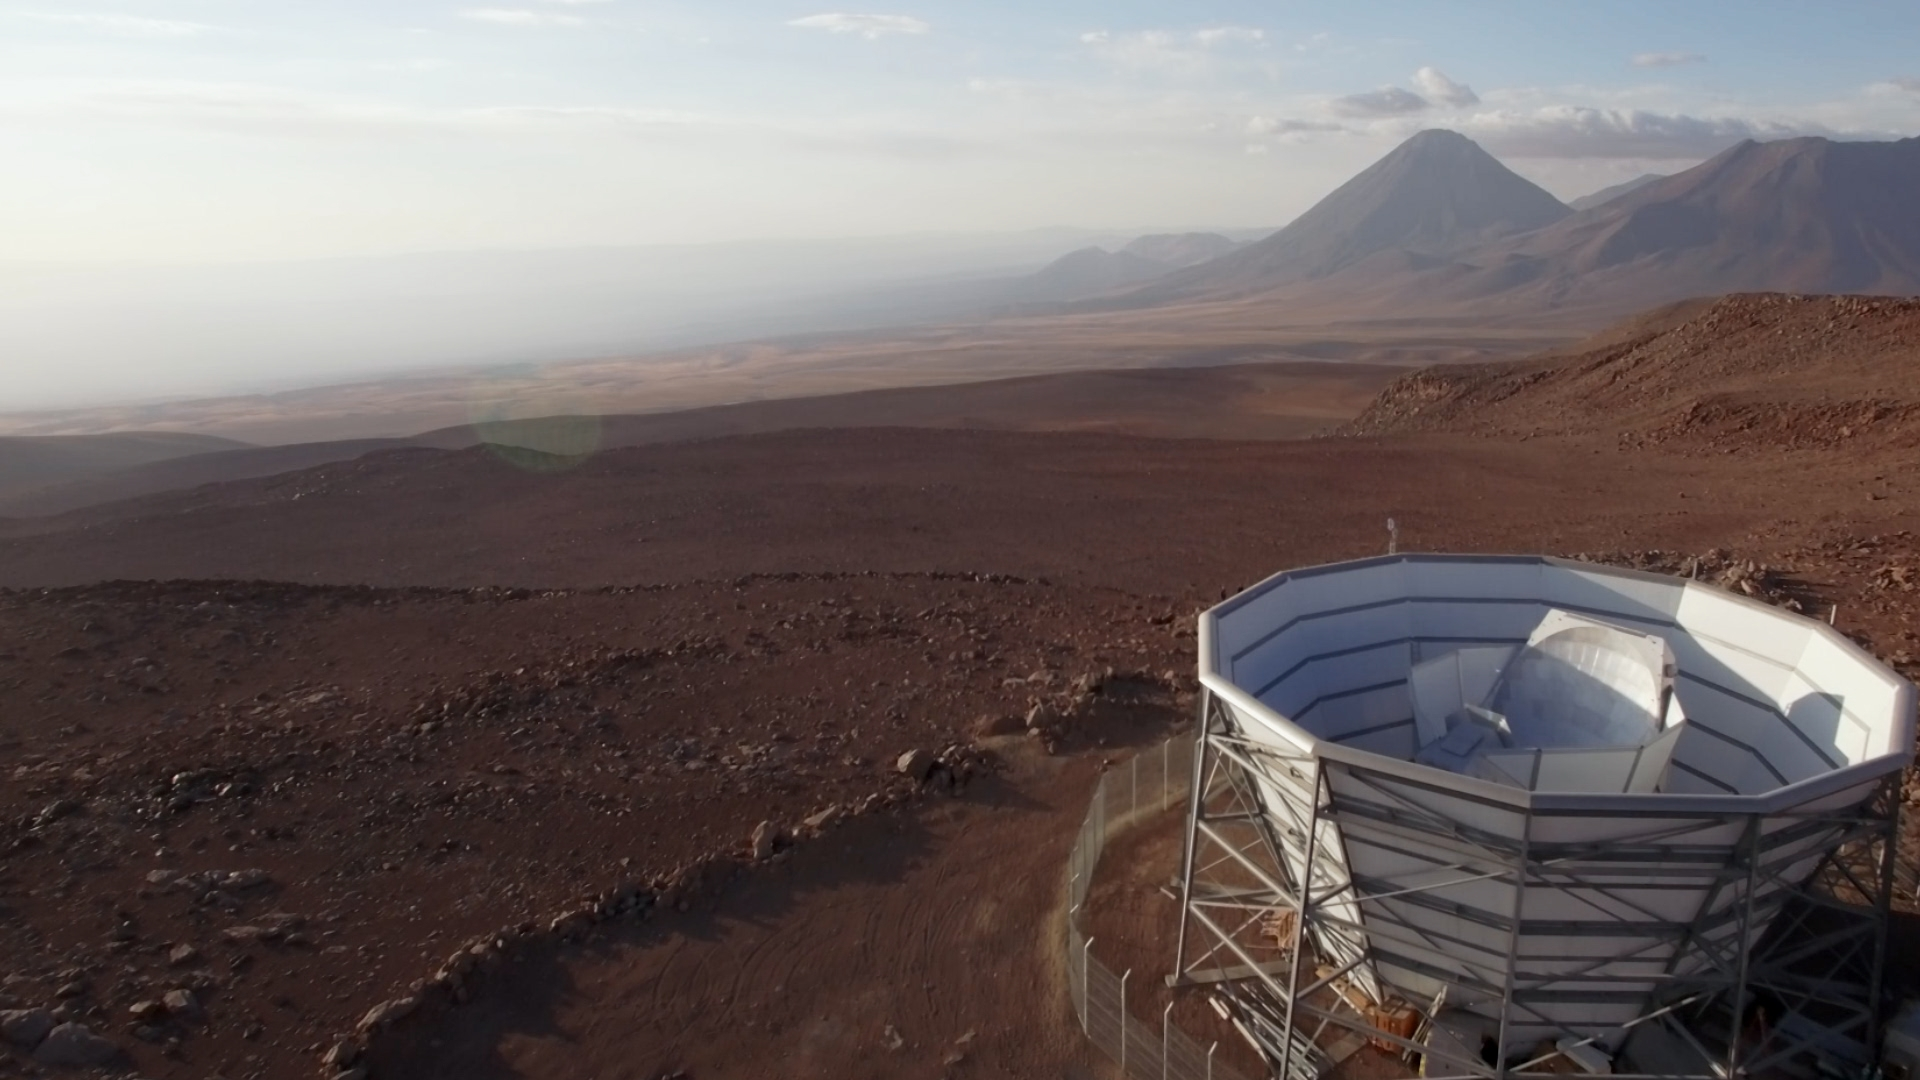
\includegraphics[height=0.15183\textwidth]{figures/telescopes/SO}%
        \vspace{-1pt}

        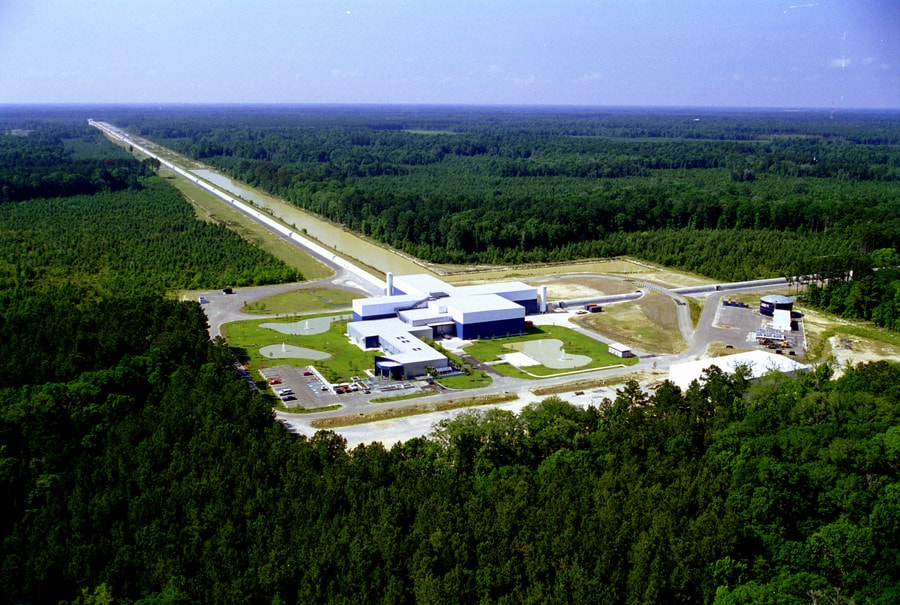
\includegraphics[height=0.18428\textwidth]{figures/telescopes/ligo}%
        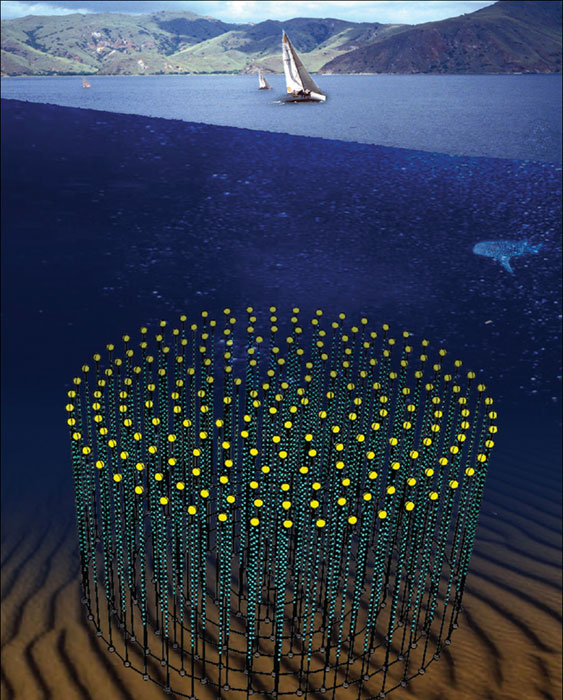
\includegraphics[height=0.18428\textwidth]{figures/telescopes/km3n}%
        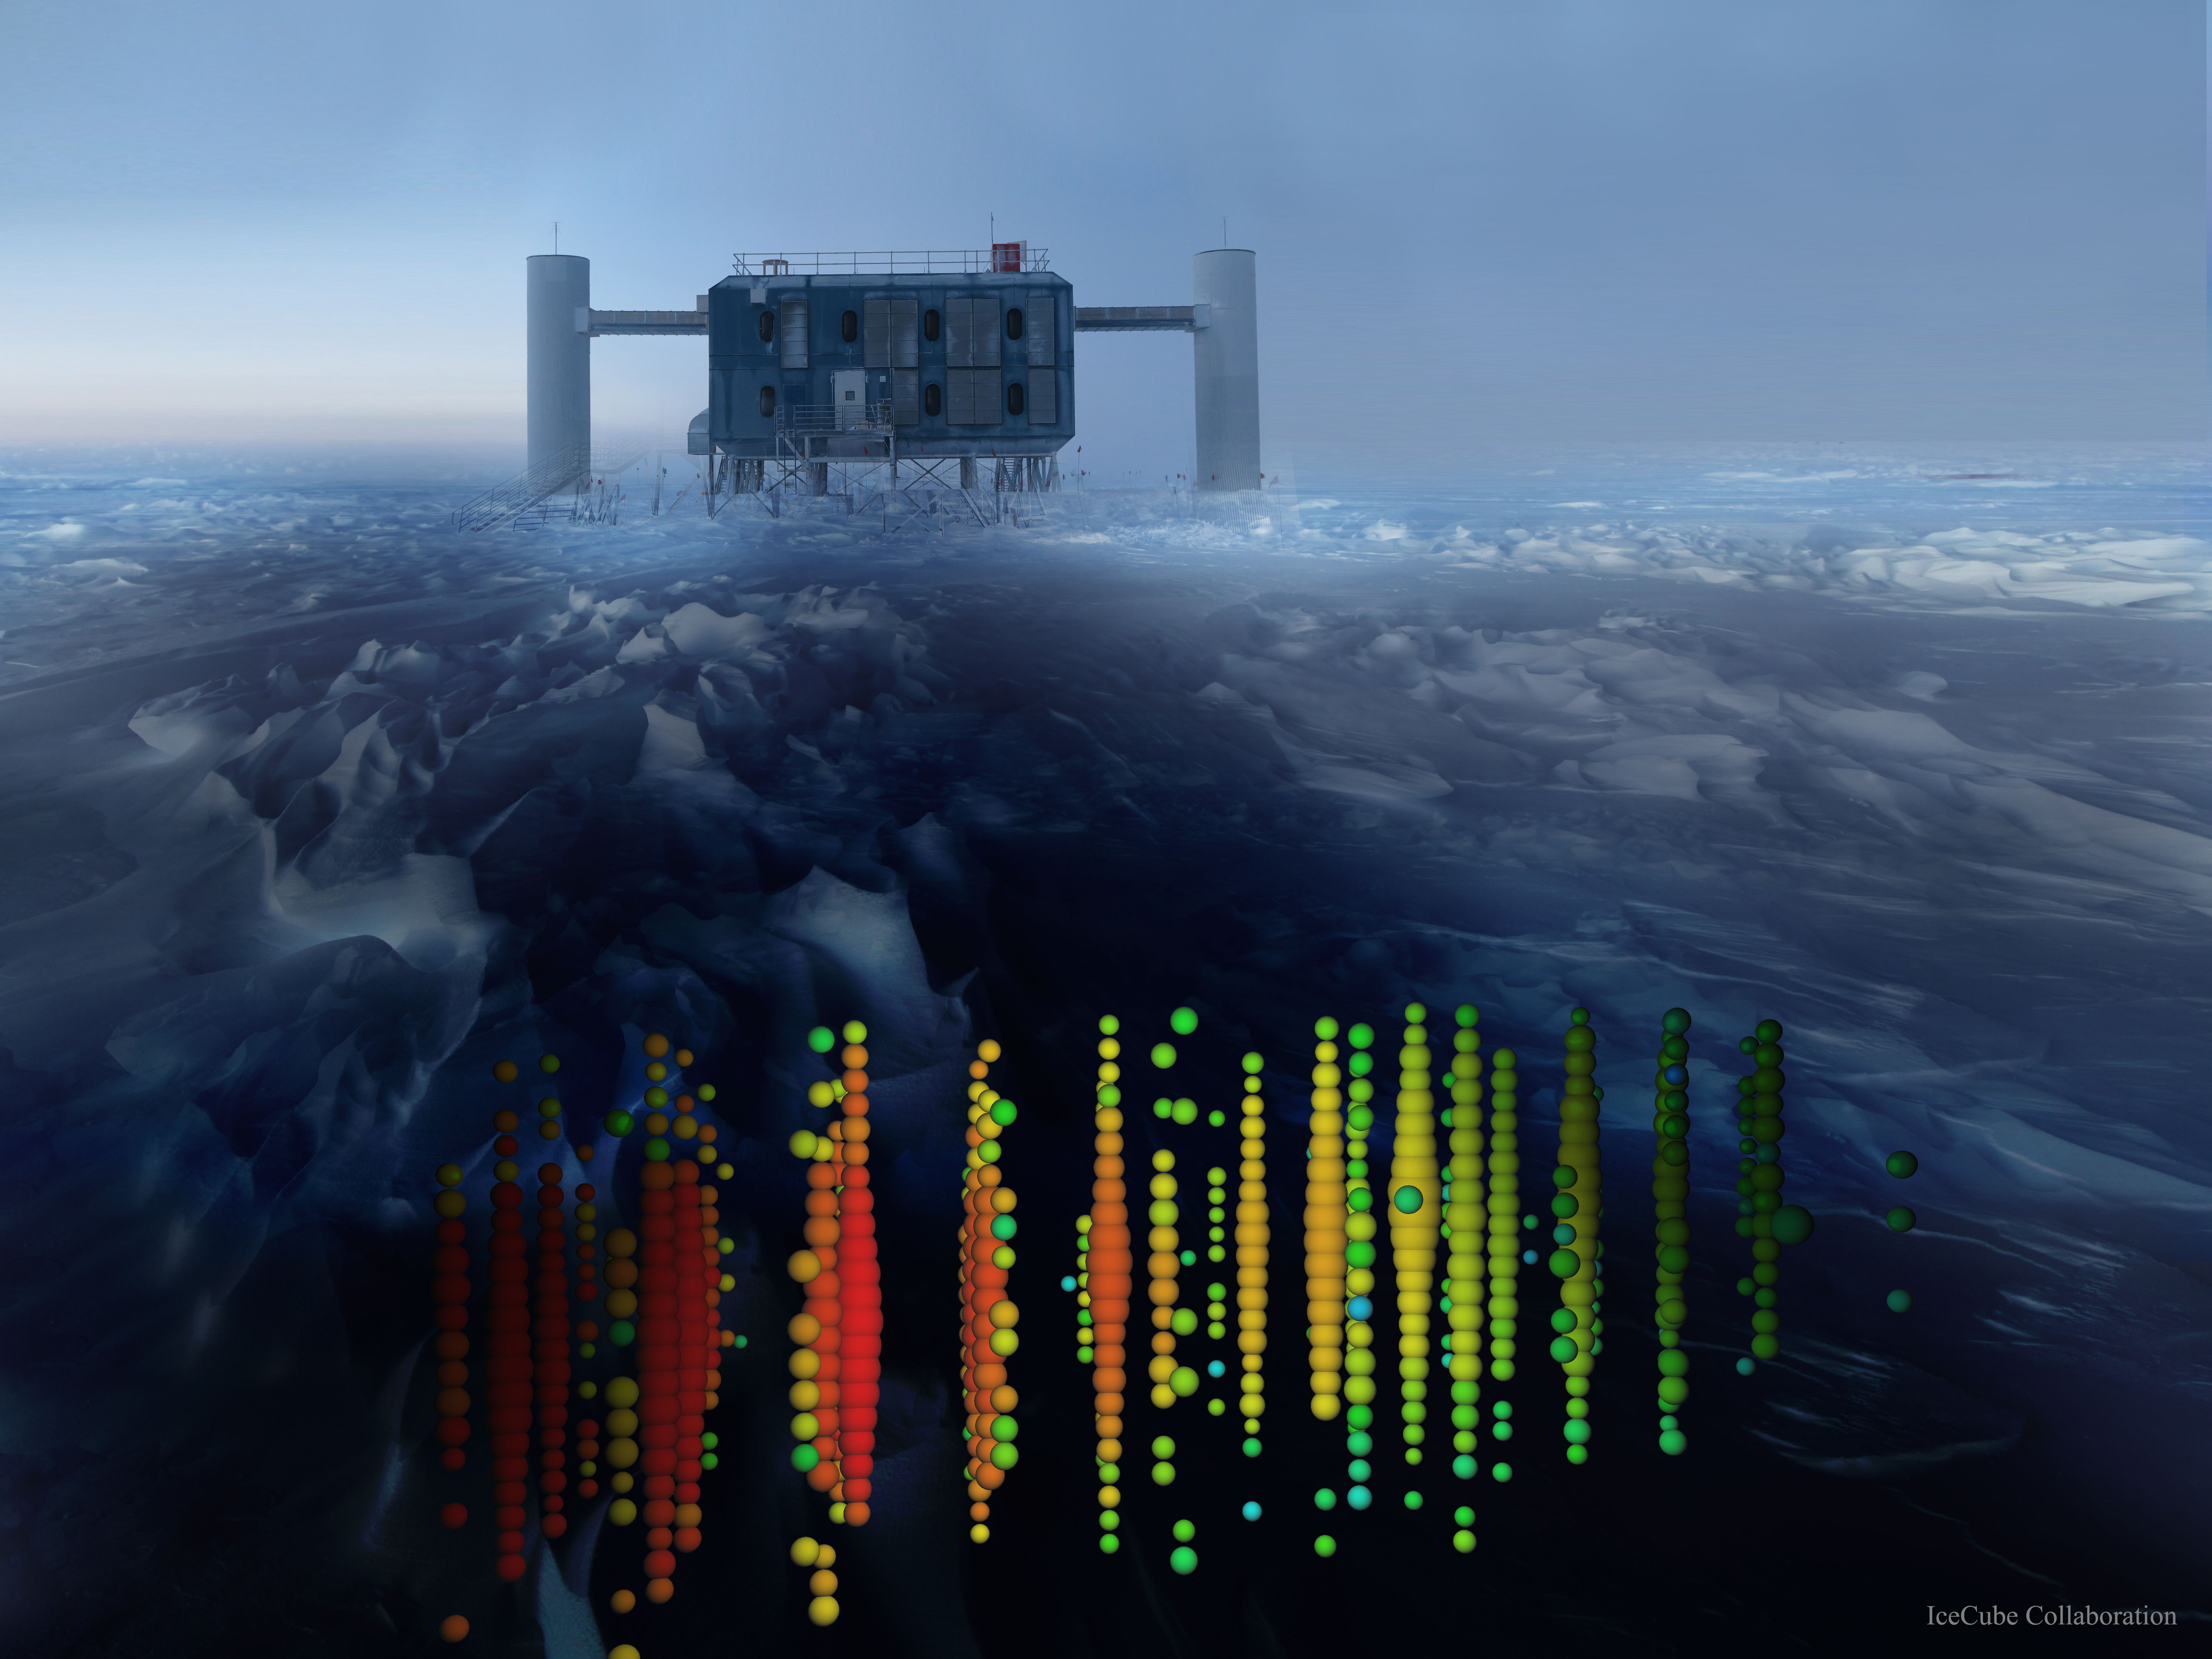
\includegraphics[height=0.18428\textwidth]{figures/telescopes/icecube}%
        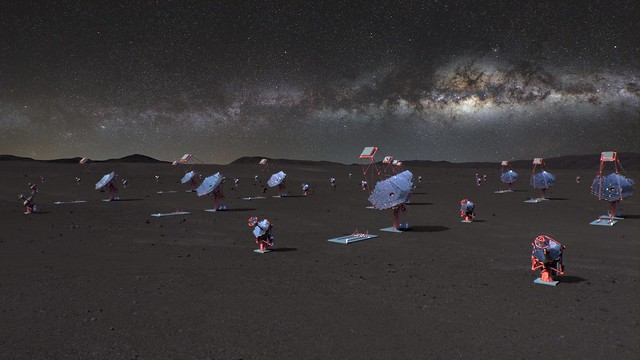
\includegraphics[height=0.18428\textwidth]{figures/telescopes/CTA}%

        \begin{itemize}
            \item We are moving from an age of \textbf{precision} cosmology to \textbf{accurate} cosmology.
            \item \textbf{Systematics} $\gtrsim$ \textbf{statistics}.
            \item Tools risk lagging behind hardware
        \end{itemize}
        
    \end{columns}
\end{frame}

\begin{frame}
    \frametitle{Tensions in cosmology}
    \begin{columns}
        \column{0.5\textwidth}
        \begin{itemize}
            \item \textbf{Data}:
                    $H_0$, $S_8$, $A_L/\Omega_K$, Li
            \item \textbf{Theory}:
                    Initial conditions, Entropy, Dark energy, dark matter, quantum gravity
            \item \textbf{Analysis}:
            \item Disentangling systematics from new physics is challenging!
            \item Almost all cosmological analyses pragmatically assume a fiducial flat $\Lambda$CDM assumption during their analyses.
            \item Unless this is resolved, we risk confirmation bias in the analysis of next-generation data.
        \end{itemize}
        \column{0.5\textwidth}
        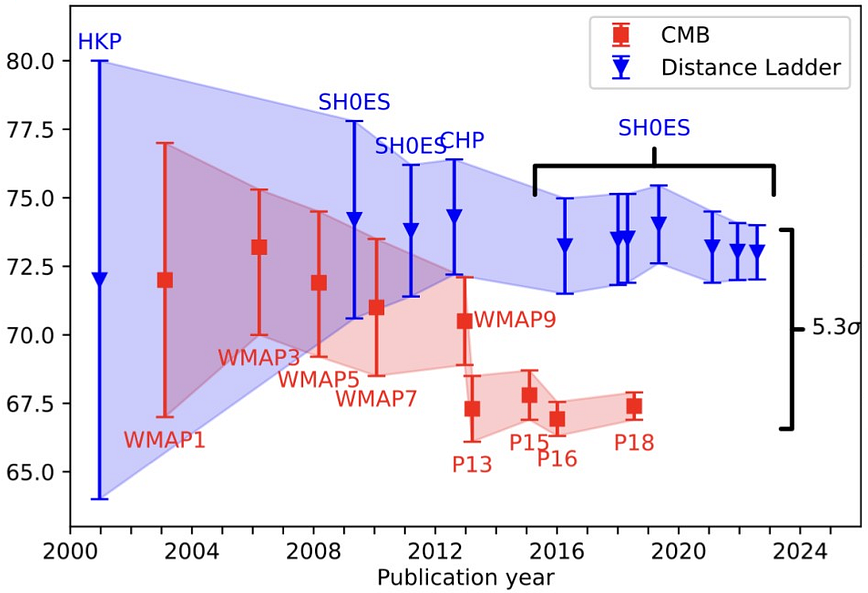
\includegraphics[height=0.45\textwidth]{figures/hubble_tension}%
        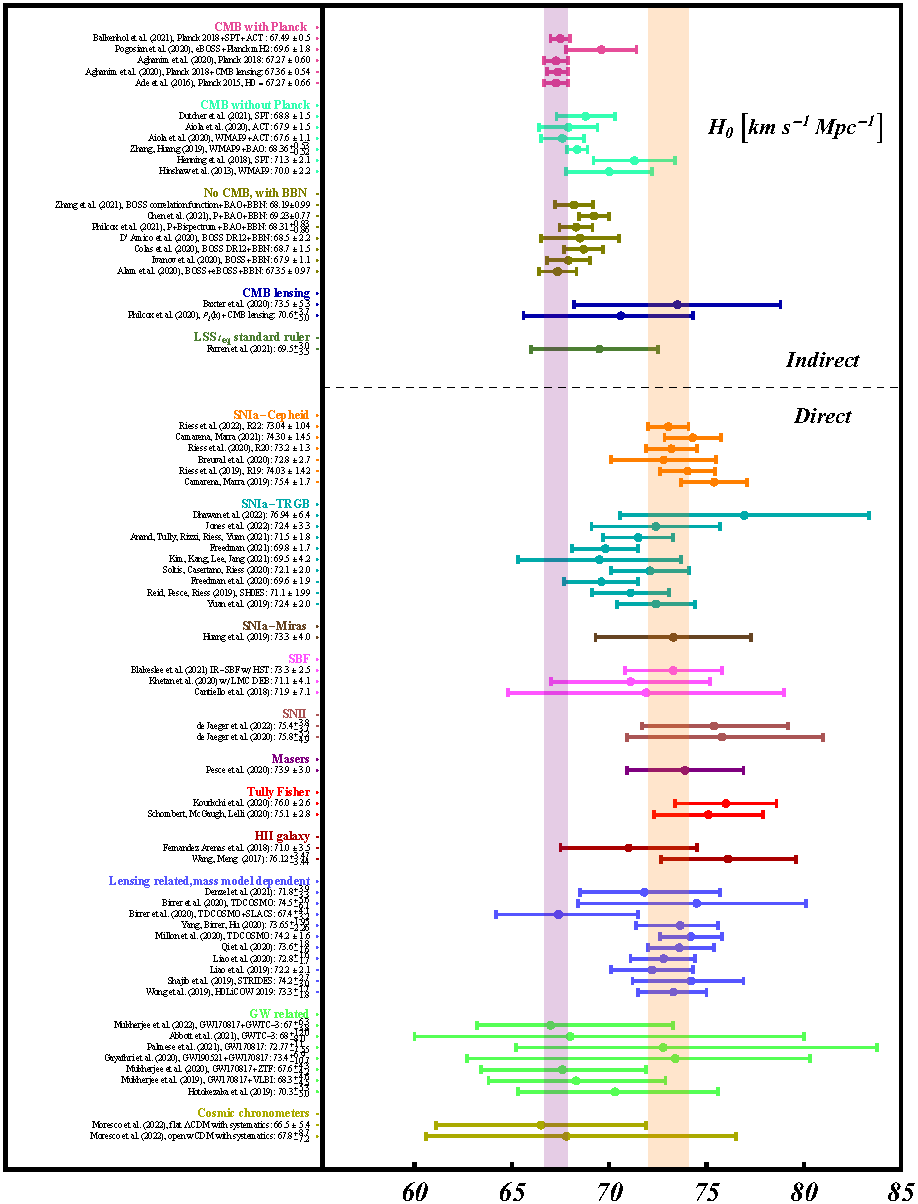
\includegraphics[height=0.45\textwidth]{figures/hubble_survey}
        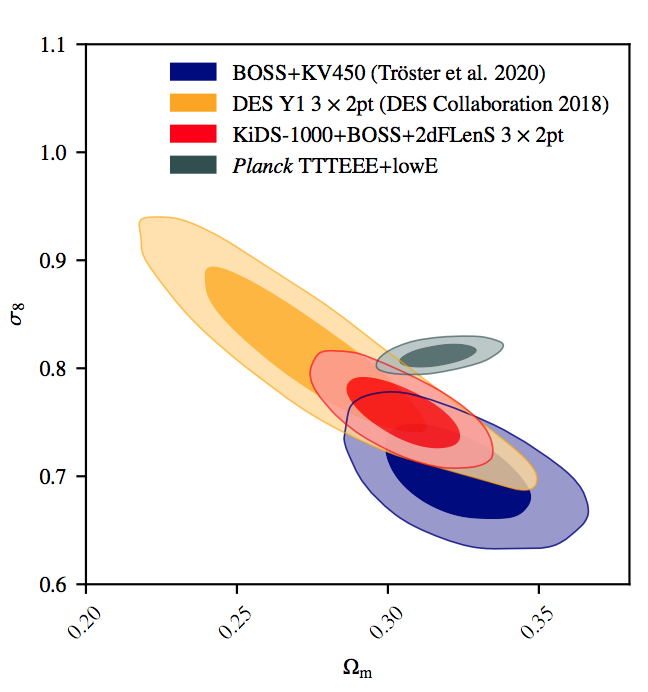
\includegraphics[height=0.5\textwidth]{figures/S8}%
        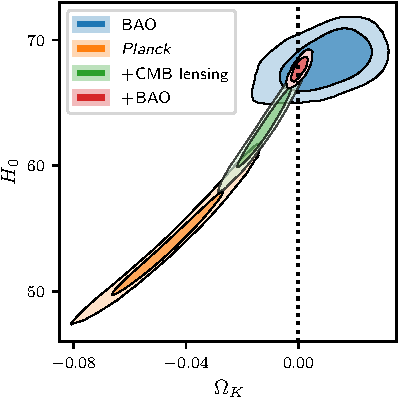
\includegraphics[height=0.5\textwidth]{figures/curvature_3}
    \end{columns}
\end{frame}

\begin{frame}
    \frametitle{Structure of talk}
    \begin{enumerate}
        \item Likelihood-based inference
        \item Nested sampling
        \item Marginal hierarchical inference
        \item Simulation-based inference
        \item Fully Bayesian Forecasts
    \end{enumerate}
\end{frame}

\begin{frame}
    \frametitle{Bayesian notation}
    \begin{itemize}
        \item A ``generative'' model $M$, with tunable parameters $\theta$, describing (compressed) data $D$.
            \begin{itemize}
                \item e.g. $M=\Lambda$CDM, $\theta=\{\Omega_b,\Omega_c, \tau, H_0, A_s, n_s\}$, $D=\{C_\ell\}$.
            \end{itemize}
        \item Described by simulation process $\theta\to D$, or likelihood $P(D|\theta,M)$.
        \item Frequentists \& Bayesians agree on the likelihood.
        \item Bayesians treat parameter space $\theta$ the same as data space $D$.
        \item Quantifying uncertainty with probability using Bayes theorem:
        \[
            \C[0]{P}(\theta|D,M) = \frac{\C[2]{P}(D|\theta,M)\C[1]{P}(\theta|M)}{\C[3]{P}(D|M)},
            \quad
            \C[0]{\text{Posterior}} = \frac{\C[2]{\text{Likelihood}}\times\C[1]{\text{Prior}}}{\C[3]{\text{Evidence}}},
            \quad
            \C[0]{\mathcal{P}}(\theta|D) = \frac{\C[2]{\mathcal{L}}(D|\theta)\C[1]{\pi}(\theta)}{\C[3]{\mathcal{Z}}(D)}.
        \]
    \item Follows from the oft-forgotten Joint (the probability of everything):
        \[
            \C[0]{\mathcal{P}}\times\C[3]{\mathcal{Z}} = \C[4]{\mathcal{J}} = \C[2]{\mathcal{L}}\times\C[1]{\pi}, \qquad \C[4]{P}(D,\theta|M) = \C[4]{\text{Joint}} = \C[4]{\mathcal{J}}  
        \]
    \item Also relevant (in many overlapping contexts) is the dimensionless ratio
\[\C[5]{r} = \frac{\C[4]{\mathcal{J}}}{\C[1]{\pi}\times\C[3]{\mathcal{Z}}} = \frac{\C[2]{\mathcal{L}}}{\C[3]{\mathcal{Z}}} = \frac{\C[0]{\mathcal{P}}}{\C[1]{\pi}}\]
    \end{itemize}
\end{frame}

\begin{frame}
    \frametitle{The three pillars of Bayesian inference}
    \vspace{-30pt}
    \begin{columns}[t]
        \column{0.33\textwidth}
        \begin{block}{Parameter estimation}
            What do the data tell us about the parameters of a model?

            \textit{e.g. the size or age of a $\Lambda$CDM universe}
            \[ \hspace{-4pt}\C[0]{P(\theta|D,M)} = \frac{\C[2]{P(D|\theta,M)} \C[1]{P(\theta|M)}}{\C[3]{P(D|M)}} \] 
            \[ \C[0]{\mathcal{P}} = \frac{\C[2]{\mathcal{L}} \times\C[1]{\pi}}{\C[3]{\mathcal{Z}}}\] 
            \[ \C[0]{\text{Posterior}} = \frac{\C[2]{\text{Likelihood}} \times\C[1]{\text{Prior}}}{\C[3]{\text{Evidence}}}\]
        \end{block}
        \column{0.3\textwidth}
        \begin{block}{Model comparison}
            How much does the data support a particular model?

            \textit{e.g. $\Lambda$CDM vs a dynamic dark energy cosmology}
            \[ \C[6]{P(M|D)} = \frac{\C[3]{P(D|M)} \C[7]{P(M)}}{\C[8]{P(D)}} \vspace{-7pt}\]
            \[ \frac{\C[3]{\mathcal{Z}_\mathcal{M}} \C[7]{\Pi_\mathcal{M}}}{\C[8]{\sum_m Z_m \Pi_m}} \]
            \[ \C[6]{\text{Posterior}} = \frac{\C[3]{\text{Evidence}} \times\C[7]{\text{Prior}}}{\C[8]{\text{Normalisation}}}\]
        \end{block}
        \column{0.33\textwidth}
        \begin{block}{Tension quantification}
            Do different datasets make consistent predictions from the same model? 
            \textit{e.g. CMB vs Type IA supernovae data}
            \[ \mathcal{R} = \frac{\C[3]{\mathcal{Z}}_{AB}}{\C[3]{\mathcal{Z}}_A\C[3]{\mathcal{Z}}_\mathcal{B}}\] 
            \[
                \begin{aligned} \log\mathcal{S} = \av[{\C[0]{\mathcal{P}}_{AB}}]{\C[2]{\log\mathcal{L}}_{AB}}&\\
                    -\av[{\C[0]{\mathcal{P}}_{A}}]{\C[2]{\log\mathcal{L}}_{A}}&\\
                    -\av[{\C[0]{\mathcal{P}}_{B}}]{\C[2]{\log\mathcal{L}}_{B}}&
                \end{aligned}
            \]
        \end{block}
    \end{columns}
\end{frame}


\begin{frame}
    \frametitle{LBI: Likelihood-based inference}
    \begin{columns}
        \column{0.5\textwidth}
        The standard approach if you are fortunate enough to have a likelihood function $\mathcal{L}(D|\theta)$: 
        e.g recent DES analysis \arxiv{2401.02929}
        \begin{enumerate}
            \item Define prior $\pi(\theta)$ 
                \begin{itemize}
                    \item spend some time being philosophical
                \end{itemize}
            \item Sample posterior $\mathcal{P}(\theta|D)$ 
                \begin{itemize}
                    \item use out-of-the-box MCMC tools such as\\ \texttt{emcee} or \texttt{MultiNest}
                    \item make some triangle plots
                \end{itemize}
            \item Optionally compute evidence $\mathcal{Z}(D)$
                \begin{itemize}
                    \item e.g. nested sampling or parallel tempering
                    \item do some model comparison (i.e. science)
                \end{itemize}
            \item Optionally talk about tensions
                \begin{itemize}
                    \item Bayes ratio (Nested Sampling)
                    \item Suspiciousness (MCMC)~\arxiv{2007.08496}
                \end{itemize}
        \end{enumerate}
        \column{0.5\textwidth}
        \hfill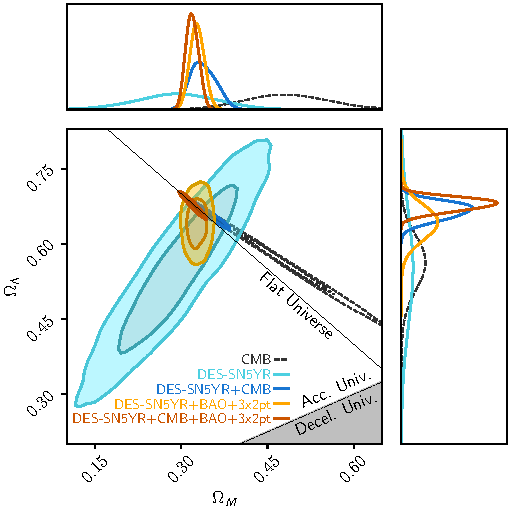
\includegraphics[width=0.6\textwidth]{figures/des_parameters.pdf}
        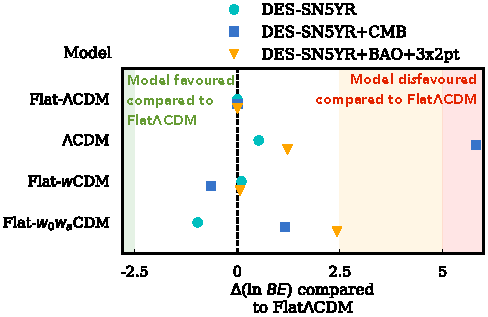
\includegraphics[width=0.5\textwidth]{figures/des_model_comparison.pdf}%
        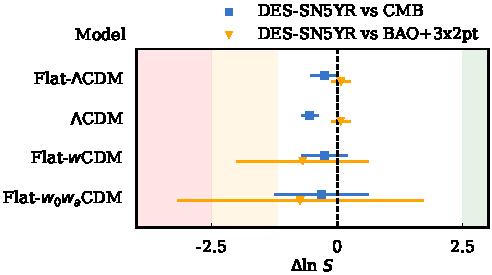
\includegraphics[width=0.5\textwidth]{figures/des_suspiciousness.pdf}
    \end{columns}
\end{frame}

\begin{frame}
    \frametitle{What is Nested Sampling?}
    \begin{itemize}
        \item Nested sampling is a radical, multi-purpose numerical tool.
        \item Given a (scalar) function $f$ with a vector of parameters $\theta$, it can be used for:
    \end{itemize}
    \vspace{-10pt}
    \begin{columns}[t]
        \column{0.3\textwidth}
        \begin{block}{Optimisation}
            \[\theta_\text{max} = \max_\theta{f(\theta)}\]
        \end{block}
        \column{0.3\textwidth}
        \begin{block}{Exploration}
            \vspace{-10pt}
            \[\text{draw/sample}\quad \theta\sim f\]
            \vspace{-15pt}
        \end{block}
        \column{0.3\textwidth}
        \begin{block}{Integration}
            \[\int f(\theta) dV \]
        \end{block}
    \end{columns}
    \begin{columns}[t]
        \column{0.33\textwidth}
        \centerline{\includegraphics[width=0.8\textwidth,page=13]{figures/himmelblau}}
        \column{0.33\textwidth}
        \centerline{\includegraphics[width=0.8\textwidth,page=15]{figures/himmelblau}}
        \column{0.33\textwidth}
        \centerline{\includegraphics[width=0.8\textwidth,page=14]{figures/himmelblau}}
    \end{columns}
\end{frame}

\begin{frame}
    \begin{columns}
        \column{0.48\textwidth}
        \begin{block}{\textbf{MCMC}}
%            \only<16>{
%                \begin{itemize}
%                    \item Single ``walker''
%                    \item Explores posterior
%                    \item Fast, if proposal matrix is tuned
%                    \item Parameter estimation, suspiciousness calculation
%                    \item Channel capacity optimised for generating posterior samples
%                \end{itemize}
%            }
        \end{block}
            \includegraphics<1>[width=\textwidth,page=16]{figures/himmelblau}%
            \includegraphics<2>[width=\textwidth,page=17]{figures/himmelblau}%
            \includegraphics<3>[width=\textwidth,page=18]{figures/himmelblau}%
            \includegraphics<4>[width=\textwidth,page=19]{figures/himmelblau}%
            \includegraphics<5>[width=\textwidth,page=20]{figures/himmelblau}%
            \includegraphics<6-15>[width=\textwidth,page=21]{figures/himmelblau}%
%        \centerline{\includegraphics<16>[width=0.5\textwidth,page=19]{figures/himmelblau}}
        \column{0.48\textwidth}
        \begin{block}<7->{\textbf{Nested sampling}}
%            \only<16>{
%                \begin{itemize}
%                    \item Ensemble of ``live points''
%                    \item Scans from prior to peak of likelihood
%                    \item Slower, no tuning required
%                    \item Parameter estimation, model comparison, tension quantification
%                    \item Channel capacity optimised for computing partition function
%                \end{itemize}
%            }
        \end{block}
            \includegraphics<7|handout:0>[width=\textwidth,page=1]{figures/himmelblau}%
            \includegraphics<8|handout:0>[width=\textwidth,page=2]{figures/himmelblau}%
            \includegraphics<9|handout:0>[width=\textwidth,page=3]{figures/himmelblau}%
            \includegraphics<10          >[width=\textwidth,page=4]{figures/himmelblau}%
            \includegraphics<11|handout:0>[width=\textwidth,page=5]{figures/himmelblau}%
            \includegraphics<12|handout:0>[width=\textwidth,page=6]{figures/himmelblau}%
            \includegraphics<13|handout:0>[width=\textwidth,page=7]{figures/himmelblau}%
            \includegraphics<14|handout:0>[width=\textwidth,page=8]{figures/himmelblau}%
            \includegraphics<15|handout:0>[width=\textwidth,page=15]{figures/himmelblau}%
%        \centerline{\includegraphics<16>[width=0.5\textwidth,page=4]{figures/himmelblau}} 
    \end{columns}
\end{frame}

\begin{frame}
    \frametitle{The nested sampling meta-algorithm: Lebesgue integration}
    \begin{columns}
        \column{0.52\textwidth}
        \begin{itemize}
            \item Full dead-point coverage of tails enables integration.
            \item Can be weighted to form posterior samples, prior samples, or anything in between.
            \item Nested sampling estimates the \textbf{density of states} and calculates partition functions
                \[Z(\beta) = \sum_i f(x_i)^\beta \Delta V_i.\]
            \item The evolving ensemble of live points allows:
                \begin{itemize}
                    \item implementations to self-tune
                    \item exploration of multimodal functions
                    \item global and local optimisation
                \end{itemize}
            %\item Interpreted as a Bayesian algorithm, it
            %    \begin{itemize}
            %        \item Computes the Bayesian evidence (model comparison)
            %        \item Produces (weighted) posterior samples (parameter estimation)
            %    \end{itemize}
        \end{itemize}
        \column{0.48\textwidth}
        \includegraphics[width=\textwidth,page=14]{figures/himmelblau}%
        %\includegraphics<1|handout:0>[width=\textwidth,page=14]{figures/himmelblau}%
        %\includegraphics<2          >[width=\textwidth,page=15]{figures/himmelblau}%
    \end{columns}
\end{frame}


\begin{frame}
    \frametitle{Implementations of Nested Sampling \arxiv{2205.15570}(NatReview)}
    %\begin{columns}
    %    \begin{column}{0.33}
    %        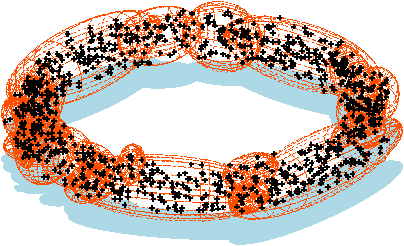
\includegraphics[width=\textwidth]{figures/multinest}
    %    \end{column} 
    %\end{columns}
    \begin{columns}[t]
        \column{0.3\textwidth}
        \texttt{MultiNest}~\arxiv{0809.3437}
        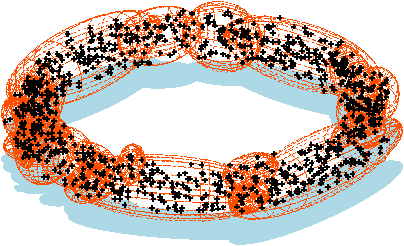
\includegraphics[width=\textwidth]{figures/multinest}
        \texttt{UltraNest}~\arxiv{2101.09604}
        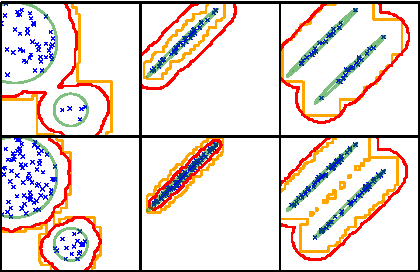
\includegraphics[width=\textwidth]{figures/radfriends}
        \column{0.4\textwidth}
        \texttt{PolyChord}~\arxiv{1506.00171}
        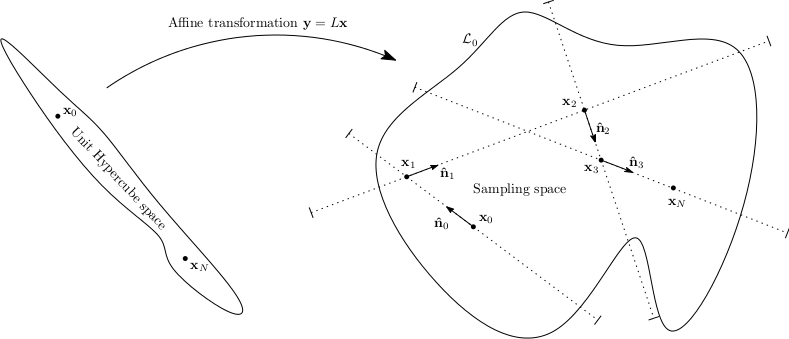
\includegraphics[width=\textwidth]{figures/polychord}
        \vfill
        \texttt{NeuralNest}~\arxiv{1903.10860}
        \begin{columns}
            \column{0.5\textwidth}
            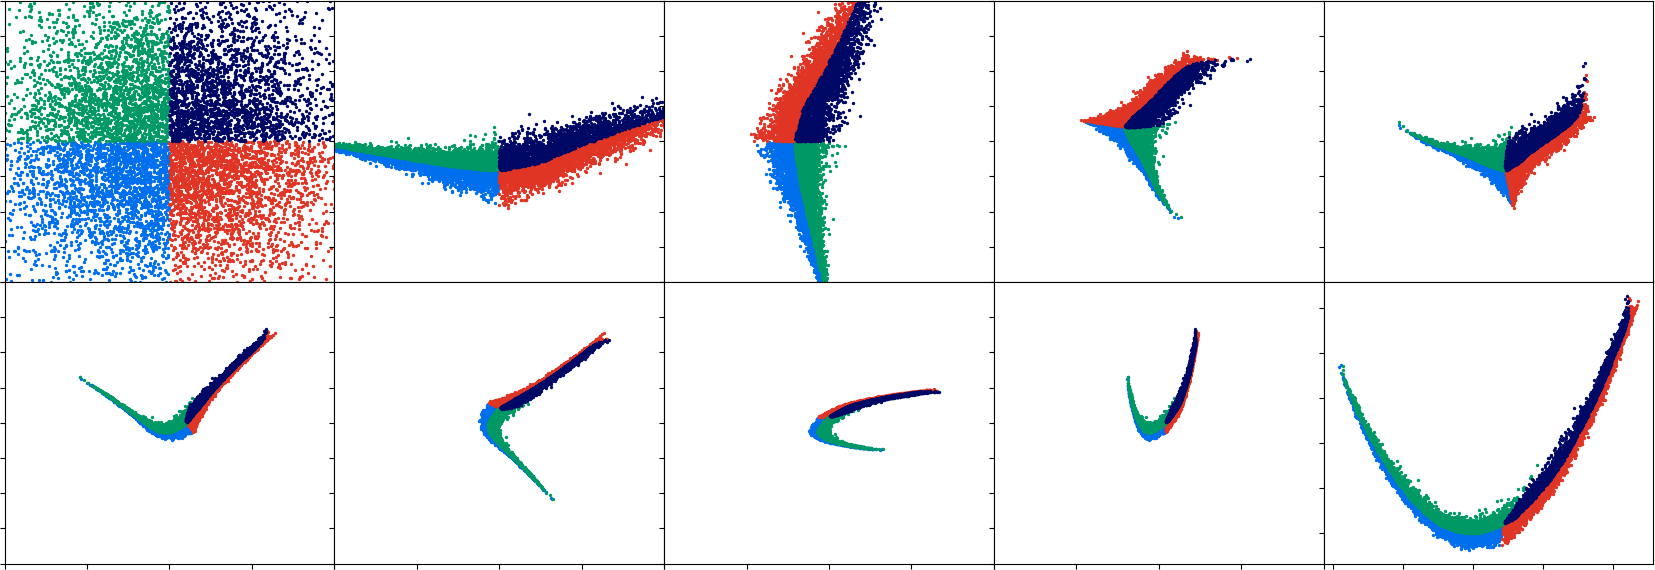
\includegraphics[width=\textwidth]{figures/rosenbrock_flow.png}
            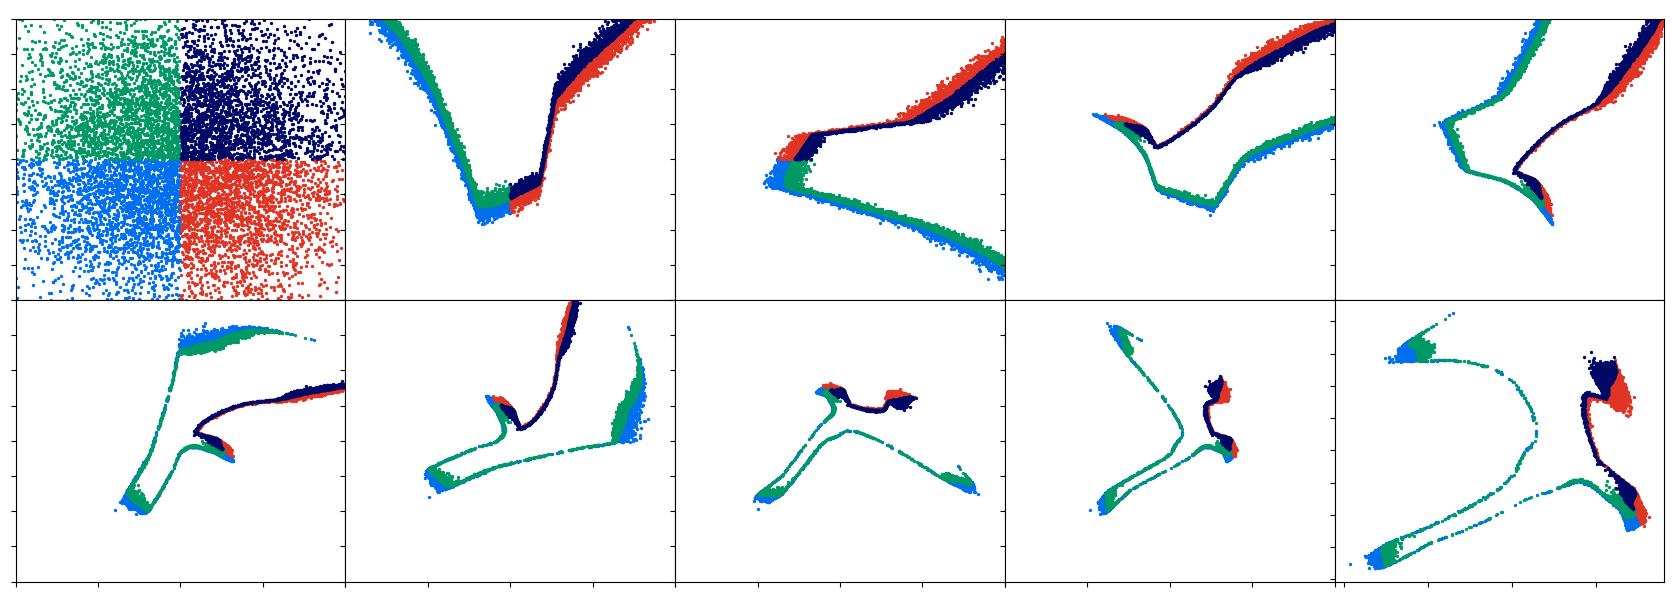
\includegraphics[width=\textwidth]{figures/himmelblau_flow.png}
            \column{0.5\textwidth}
            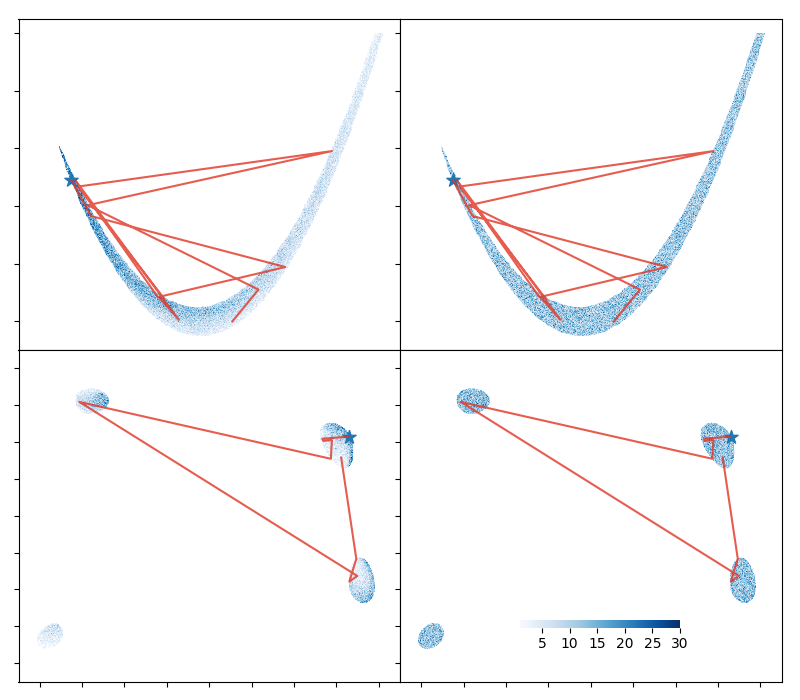
\includegraphics[width=\textwidth]{figures/chains.png}
        \end{columns}
        \texttt{nessai}~\arxiv{2102.11056} \texttt{nora}~\arxiv{2305.19267}
        \vfill
        \column{0.3\textwidth}
        \texttt{DNest}~\arxiv{1606.03757}
        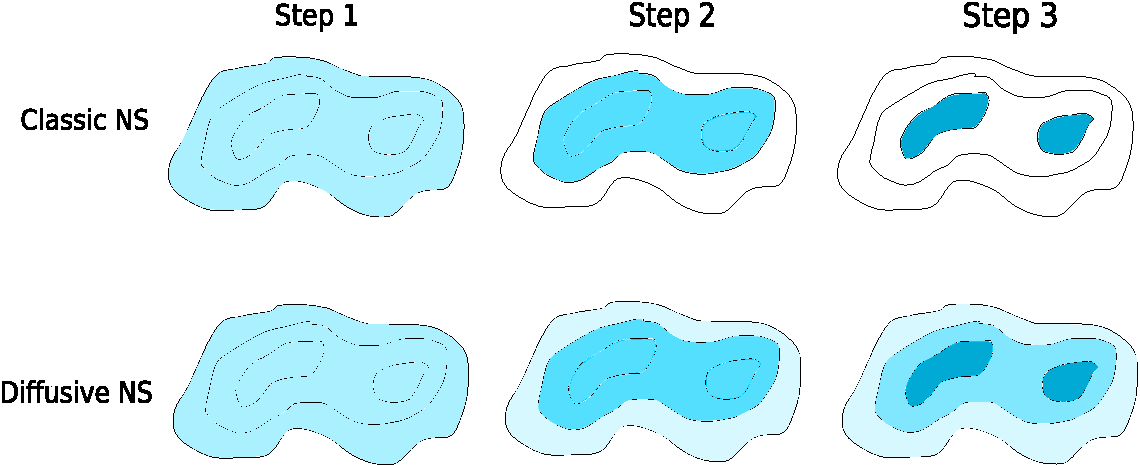
\includegraphics[width=\textwidth]{figures/dnest}
        \texttt{ProxNest}~\arxiv{2106.03646}
        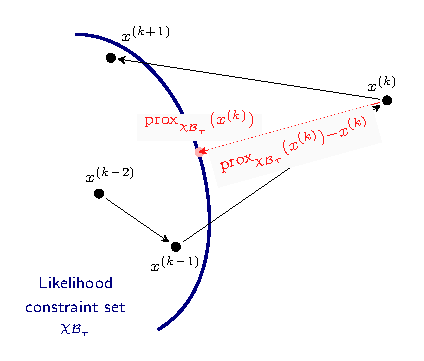
\includegraphics[width=\textwidth]{figures/proxnest_diagram}
        \texttt{dynesty}~\arxiv{1904.02180} 
        \vfill
    \end{columns}
\end{frame}

\begin{frame}
    \frametitle{Standard uses of nested sampling}
    %\only<1>{\student{adam_ormondroyd}{Adam Ormondroyd}{PhD}}
    %\only<2>{\student{metha_prathaban}{Metha Prathaban}{PhD}}
    \begin{columns}
        \column{0.55\textwidth}
        \vspace{-10pt}
        \begin{itemize}
            \item Battle-tested in Bayesian cosmology on
                \begin{itemize}
                    \item Parameter estimation: multimodal alternative to MCMC samplers.
                    \item Model comparison: using integration to compute the Bayesian evidence
                    \item Tension quantification: using deep tail sampling and suspiciousness computations.
                \end{itemize}
            \item Plays a critical role in major cosmology pipelines: Planck, DES, KiDS, BAO, SNe.
            \item The default $\Lambda$CDM cosmology is well-tuned to have Gaussian-like posteriors for CMB data. 
            \item Less true for alternative cosmologies/models and orthogonal datasets, so nested sampling crucial.
            \item Also used in Gravitational Waves \& Exoplanets
            \item Often taken as ``ground truth to beat''.
        \end{itemize}
        \column{0.45\textwidth}
        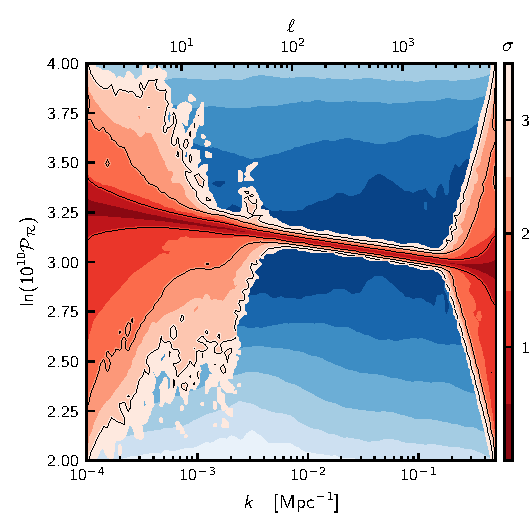
\includegraphics[width=0.49\textwidth]{figures/pps_both}
        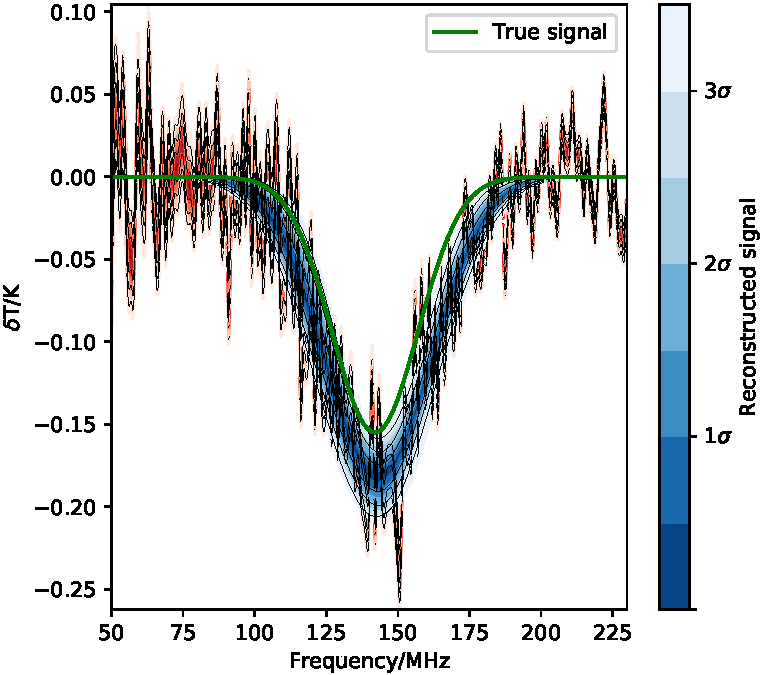
\includegraphics[width=0.49\textwidth]{figures/reach_fit-cropped.pdf}
        %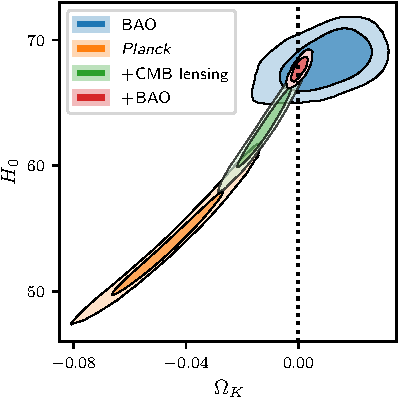
\includegraphics[width=0.49\textwidth]{figures/curvature_3}
        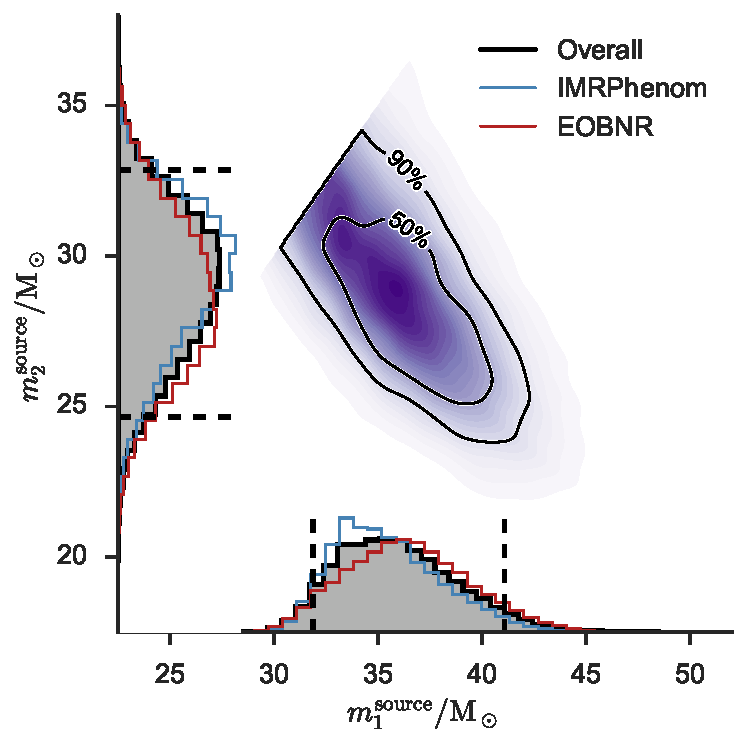
\includegraphics[width=0.49\textwidth]{figures/ligo_m1_m2.pdf}
        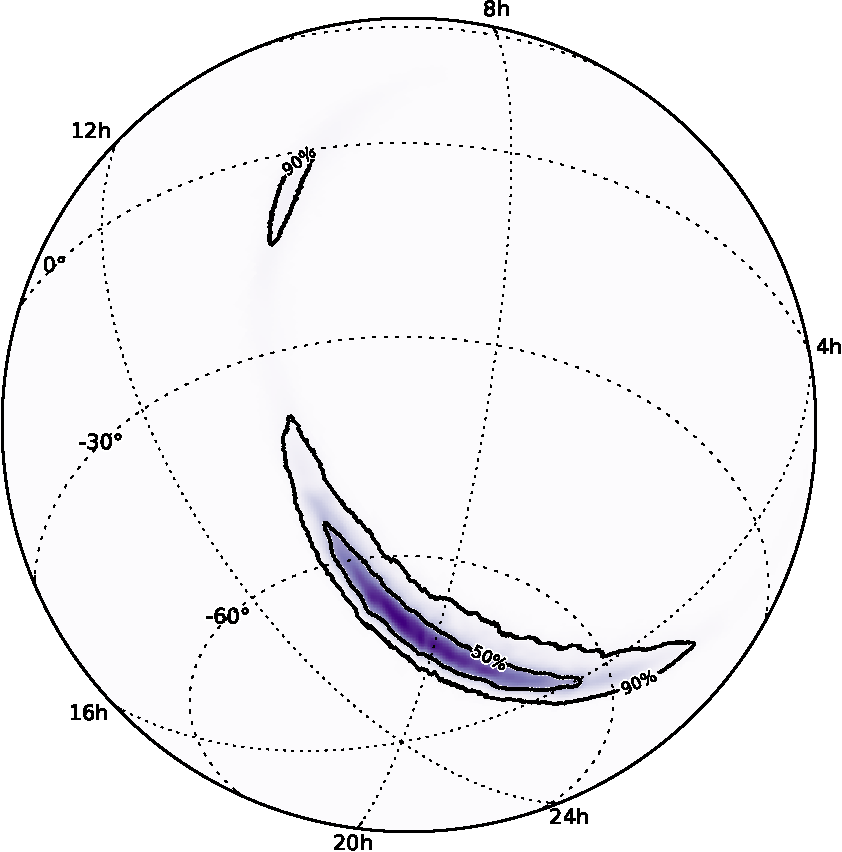
\includegraphics[width=0.49\textwidth]{figures/ligo_lambert-skymap.pdf}
    \end{columns}
\end{frame}

\begin{frame}
    \frametitle{Marginal inference}
    \student{harry_bevins}{Harry Bevins}{PhD$\to$JRF}
    \begin{columns}
        \column{0.5\textwidth}
        \begin{itemize}
            \item Many cosmological likelihoods come with nuisance parameters that have limited relevance for onward inference.
            \item Notation: \only<1>{CMB cosmology} \only<2>{GW cosmology}
                \begin{itemize}
                    \item[$\mathcal{L}$] Likelihood \hfill (e.g. \only<1>{\texttt{plik}}\only<2>{LAL}),
                    \item[$D$] Data \hfill (e.g. \only<1>{CMB}\only<2>{GW170817}),
                    \item[$\theta$] Cosmological parameters \hfill (e.g. \only<1>{$\Omega_m$}, $H_0$\ldots),
                    \item[$\alpha$] Nuisance parameters \hfill (e.g. \only<1>{$A_\text{planck}$}\only<2>{$m_1$, $m_2$}\ldots),
                    \item[$M$] Model \hfill (e.g. $\Lambda$CDM).
                \end{itemize}
            \item Some marginal statistics (e.g. marginal means, posteriors\ldots) are easy to compute.
            \item More machinery is needed for e.g. nuisance marginalised likelihoods and marginal KL divergences $\mathcal{D}_\text{KL}$.
        \end{itemize}
        \column{0.5\textwidth}
\vspace{10pt}
        \includegraphics<1>{figures/planck_2018_plik.pdf}%
        \includegraphics<2>[width=\textwidth]{figures/standardsirens}
        \includegraphics<2>[width=\textwidth]{figures/graveyard}
    \end{columns}
\end{frame}

\begin{frame}
\frametitle{Nuisance marginalised likelihoods: Theory {\small\arxiv{2207.11457}}}
    \student{harry_bevins}{Harry Bevins}{PhD$\to$JRF}
    \begin{columns}[t]
        \column{0.5\textwidth}
        \begin{itemize}
            \item Bayes theorem
                \begin{align}
                    \C[2]{\mathcal{L}}(\theta,\alpha) 
                    \times 
                    \C[1]{\pi}(\theta,\alpha) &= 
                    \C[0]{\mathcal{P}}(\theta,\alpha)
                    \times
                    \C[3]{\mathcal{Z}}\\
                    \C[2]{\text{Likelihood}}
                    \times
                    \C[1]{\text{Prior}}
                    &=
                    \C[0]{\text{Posterior}}
                    \times
                    \C[3]{\text{Evidence}}
                    \nonumber
                \end{align}
                \small{$\alpha$: nuisance parameters, $\theta$: cosmo parameters.}
            \item Marginal Bayes theorem
                \begin{equation}
                    \C[2]{\mathcal{L}}(\theta) 
                    \times 
                    \C[1]{\pi}(\theta) = 
                    \C[0]{\mathcal{P}}(\theta)
                    \times
                    \C[3]{\mathcal{Z}}
                \end{equation}
            \item Non-trivially gives \textbf{nuisance-free likelihood}
                \begin{equation}
                    \boxed{
                        \C[2]{\mathcal{L}}(\theta) 
                        = 
                        \frac{
                            \C[0]{\mathcal{P}}(\theta)
                            \C[3]{\mathcal{Z}}
                        }{
                            \C[1]{\pi}(\theta)
                        }
                    }
                    =
                    \frac{
                        \int \C[2]{\mathcal{L}}(\theta,\alpha) \C[1]{\pi}(\theta,\alpha) d{\alpha}
                    }
                    {
                        \int \C[1]{\pi}(\theta,\alpha) d{\alpha}
                    }
                \end{equation}
        \end{itemize}
        \column{0.5\textwidth}
        \textbf{Key properties}
        \begin{itemize}
            \item Given datasets $A$ and $B$, each with own nuisance parameters $\alpha_A$ and $\alpha_B$:
            \item If you use $\mathcal{L}_A(\theta)$, you get the same (marginal) posterior and evidence if you had run with nuisance parameters $\alpha_A$ (ditto $B$).
            \item If you run inference on $\mathcal{L}_A(\theta)\times\mathcal{L}_B(\theta)$, you get the same (marginal) posterior and evidence if you had run with all nuisance parameters $\alpha_A$, $\alpha_B$ on.
            \item[] \textit{(weak marginal consistency requirements on joint $\pi(\theta,\alpha_A,\alpha_B)$ and marginal priors)}
        \end{itemize}
    \end{columns}
\end{frame}

\begin{frame}
    \frametitle{Nuisance marginalised likelihoods: Practice~{\small\arxiv{2205.12841}}}
    \student{harry_bevins}{Harry Bevins}{PhD$\to$JRF}
    \begin{columns}
        \column{0.6\textwidth}
        \begin{columns}
            \column{0.3\textwidth}
            \[
                \boxed{
                    \C[2]{\mathcal{L}}(\theta) 
                    = 
                    \frac{
                        \C[0]{\mathcal{P}}(\theta)
                        \C[3]{\mathcal{Z}}
                    }{
                        \C[1]{\pi}(\theta)
                    }
                }
            \]
            \column{0.7\textwidth}
            \begin{itemize}
                \item To compute the nuisance marginalised likelihood, need:
                    \begin{enumerate}
                        \item Bayesian evidence $\C[3]{\mathcal{Z}}$
                        \item Marginal prior and posterior \textbf{densities}
                    \end{enumerate}
            \end{itemize}
        \end{columns}
            \begin{enumerate}
                \item Bayesian evidence $\C[3]{\mathcal{Z}}$:                              g
                    \begin{itemize}
                        \item Nested sampling
                        \item Parallel tempering (pocomc, ptmcmc)
                        \item Sequential Monte Carlo (SMC)
                        \item MCEvidence
                    \end{itemize}
                \item Marginal prior $\C[1]{\pi}(\theta)$ and posterior $\C[0]{\mathcal{P}}(\theta)$ densities:
                    \begin{itemize}
                        \item Histograms of samples
                        \item Kernel density estimation
                        \item Normalising flows / Diffusion models
                        \item \ldots
                    \end{itemize}
            \end{enumerate}
        \begin{itemize}
            %\item Combination termed \texttt{margarine} \arxiv{2205.12841}
            \item Emulators usually much faster than original likelihoods
            \item \texttt{margarine}: PyPI, \href{https://github.com/htjb/margarine}{github.com/htjb/margarine}
        \end{itemize}

        \column{0.4\textwidth}
        \begin{tikzpicture}[
                rednode/.style={rectangle, draw=red!60, fill=red!5, very thick, minimum size=5mm},
                bluenode/.style={rectangle, draw=blue!60, fill=blue!5, very thick, minimum size=5mm},
                greennode/.style={rectangle, draw=green!60, very thick, minimum size=5mm},
                node distance=0.5cm,
                remember picture, overlay
            ]
            \node<1->[bluenode, xshift=0.5\textwidth, yshift=-0.25\textwidth](likelihood) at (current page.north)  {$ \mathcal{L}(\theta,\alpha)$};
            \node<1->[bluenode, right = of likelihood.east](prior) {$ \pi(\theta,\alpha)$};

            \coordinate<1-> (likelihoodprior) at ($(likelihood.south)!0.5!(prior.south)$);

            \node<2->[rednode, below = of likelihoodprior](nestedsampling) {Nested Sampling};
            \draw<2->[->](likelihood.south) -- (likelihood|-nestedsampling.north);
            \draw<2->[->](prior.south) -- (prior|-nestedsampling.north);

            \node<3->[bluenode, below = of nestedsampling](posterior) {$ \{\theta,\alpha\}_\mathcal{P}$};
            \draw<3->[->](nestedsampling.south-|posterior) -- (posterior.north);
            \node<4->[bluenode, left = of posterior.west](evidence) {$ \mathcal{Z}$};
            \draw<4->[->](nestedsampling.south-|likelihood) -- (evidence.north);
            \node<5->[bluenode, right = of posterior.east](priorSamples) {$ \{\theta,\alpha\}_\pi$};
            \draw<5->[->](nestedsampling.south-|prior) -- (priorSamples.north);

            \coordinate<5-> (posteriorprior) at ($(posterior.south)!0.5!(priorSamples.south)$);

            \node<6->[rednode, below = of posteriorprior](margarine)  {Density Estimation};

            \draw<6->[->](posterior.south) -- (margarine.north-|posterior.east);
            \draw<6->[->](priorSamples.south) -- (margarine.north-|priorSamples.west);

            \node<7->[bluenode, below = of posterior|-margarine.south](marginalPosterior) {$ \mathcal{P}(\theta)$};


            \draw<7->[->](margarine.south-|marginalPosterior.east) -- (marginalPosterior.north);


            \node<8->[bluenode, below = of marginalPosterior.south-|margarine.south-|priorSamples](marginalPrior) {$ \pi(\theta)$};
            \draw<8->[->](margarine.south-|priorSamples.west) -- (marginalPrior.north);


            \node<9->[bluenode, below = of marginalPosterior](marginalLikelihood) {$ \mathcal{L}(\theta)$};


            \draw<9->[->](evidence.south) -- (marginalLikelihood.west);
            \draw<9->[->](marginalPosterior.south) -- (marginalLikelihood.north);
            \draw<9->[->](marginalPrior.west) -- (marginalLikelihood.east);

            \node<10->[greennode,behind path,fit=(nestedsampling) (marginalPosterior) (priorSamples) (evidence),] {};

        \end{tikzpicture}
    \end{columns}
\end{frame}

\begin{frame}
    \frametitle{Nuisance marginalised likelihoods: Example uses}
    \begin{itemize}
        \item Library of pre-trained bijectors to be used as priors/emulators/nuisance marginalised likelihoods (DiRAC allocation \texttt{unimpeded})
        \item e.g. easy to apply a \textit{Planck}/DES/HERA/JWST prior or likelihood to your existing MCMC chains without needing to install the whole cosmology machinery.
        \item Hierarchical modelling:
            \begin{itemize}
                \item Usually, have $N$ objects, each with nuisance parameters $\alpha_i$, and shared parameters of interest $\theta$.

                \item Likelihood $\C[2]{\mathcal{L}}(\{D_i\}|\theta,\{\alpha_i\}) = \prod_i^N \C[2]{\mathcal{L}}_i(D_i|\theta,\alpha_i)$ has  $N\times \texttt{len}(\alpha_i) + \texttt{len}(\theta)$ parameters
                \item Instead, break problem down into $N$ runs on $\texttt{len}(\theta) + \texttt{len}(\alpha_i)$ parameters, and one final one on $\texttt{len}(\theta)$ parameters, using nuisance marginal likelihoods $\mathcal{L}_i(\theta)$.
                \item In addition to computational tractability, also can perform model comparison with nuisance marginalised likelihoods.
            \end{itemize}
    \end{itemize}
\end{frame}

\begin{frame}
    \frametitle{SBI: Simulation-based inference}
    \begin{columns}
        \column{0.5\textwidth}
\vspace{-10pt}
        \begin{itemize}
            \item Only have access to a forward model $\theta \rightarrow D$.
            \item $(\theta,D)$ plane gives a more expansive theoretical view of inference.
            \item Forward model defines \emph{implicit} likelihood~$\C[2]{\mathcal{L}}$:
            \item Simulator generates samples from $\C[2]{\mathcal{L}}(D|\theta)$.
            \item With a prior $\C[1]{\pi}(\theta)$ can generate samples from joint distribution~$\C[4]{\mathcal{J}}(\theta,D)=\C[2]{\mathcal{L}}(D|\theta)\pi(\theta)$\\\hfill \emph{the ``probability of everything''}.
            \item Task of SBI is then to go from joint~$\C[4]{\mathcal{J}}$ samples to posterior $\C[0]{\mathcal{P}}(\theta|D)$ and evidence $\C[3]{\mathcal{Z}}(D)$ -- and possibly likelihood $\C[2]{\mathcal{L}}(D|\theta)$.
            \item Present SotA: NPE, NLE, NJE, NRE
            \item SBI \& forward modelling force us to think about data space~$D$ \& parameter space~$\theta$.
        \end{itemize}
        \column{0.5\textwidth}
        \includegraphics<1>[page=1, width=\textwidth]{figures/sbi_parameter_estimation.pdf}%
        \includegraphics<2>[page=2, width=\textwidth]{figures/sbi_parameter_estimation.pdf}%
        \includegraphics<3>[page=3, width=\textwidth]{figures/sbi_parameter_estimation.pdf}%
        \includegraphics<4>[page=4, width=\textwidth]{figures/sbi_parameter_estimation.pdf}%
        \includegraphics<5>[page=5, width=\textwidth]{figures/sbi_parameter_estimation.pdf}%
        \includegraphics<6>[page=6, width=\textwidth]{figures/sbi_parameter_estimation.pdf}%
        \includegraphics<7>[page=7, width=\textwidth]{figures/sbi_parameter_estimation.pdf}%
        \includegraphics<8>[page=8, width=\textwidth]{figures/sbi_parameter_estimation.pdf}%
        \includegraphics<9>[page=9, width=\textwidth]{figures/sbi_parameter_estimation.pdf}%
        \includegraphics<10>[page=10, width=\textwidth]{figures/sbi_parameter_estimation.pdf}%
        \includegraphics<11>[page=11, width=\textwidth]{figures/sbi_parameter_estimation.pdf}%
        \includegraphics<12>[page=12, width=\textwidth]{figures/sbi_parameter_estimation.pdf}%
        \includegraphics<13>[page=13, width=\textwidth]{figures/sbi_parameter_estimation.pdf}%
        \includegraphics<14>[page=14, width=\textwidth]{figures/sbi_parameter_estimation.pdf}%
        \includegraphics<15>[page=15, width=\textwidth]{figures/sbi_parameter_estimation.pdf}%
        \includegraphics<16>[page=16, width=\textwidth]{figures/sbi_parameter_estimation.pdf}%
        \includegraphics<17>[page=17, width=\textwidth]{figures/sbi_parameter_estimation.pdf}%
        \includegraphics<18>[page=18, width=\textwidth]{figures/sbi_parameter_estimation.pdf}%
        \includegraphics<19>[page=19, width=\textwidth]{figures/sbi_parameter_estimation.pdf}%
        \includegraphics<20>[page=20, width=\textwidth]{figures/sbi_parameter_estimation.pdf}%
        \includegraphics<21>[page=21, width=\textwidth]{figures/sbi_parameter_estimation.pdf}%
    \end{columns}
\end{frame}

\begin{frame}
    \frametitle{Why SBI?}
    \begin{columns}
        \column{0.6\textwidth}
        SBI is useful because:
        \begin{enumerate}
            \item If you don't have a likelihood, you can still do inference
                \begin{itemize}
                    \item The usual case beyond CMB cosmology
                \end{itemize}
            \item Faster than LBI
                \begin{itemize}
                    \item emulation -- also applies to LBI in principle
                \end{itemize}
            \item No need to pragmatically encode fiducial cosmologies
                \begin{itemize}
                    \item Covariance computation implicitly encoded in simulations
                \end{itemize}
            \item Equips AI/ML with Bayesian interpretability
            \item Lower barrier to entry than LBI
                \begin{itemize}
                    \item Much easier to forward model a systematic
                    \item Emerging set of plug-and-play packages
                    \item For this reason alone, it will come to dominate scientific inference
                \end{itemize}
        \end{enumerate}

        \column{0.4\textwidth}
        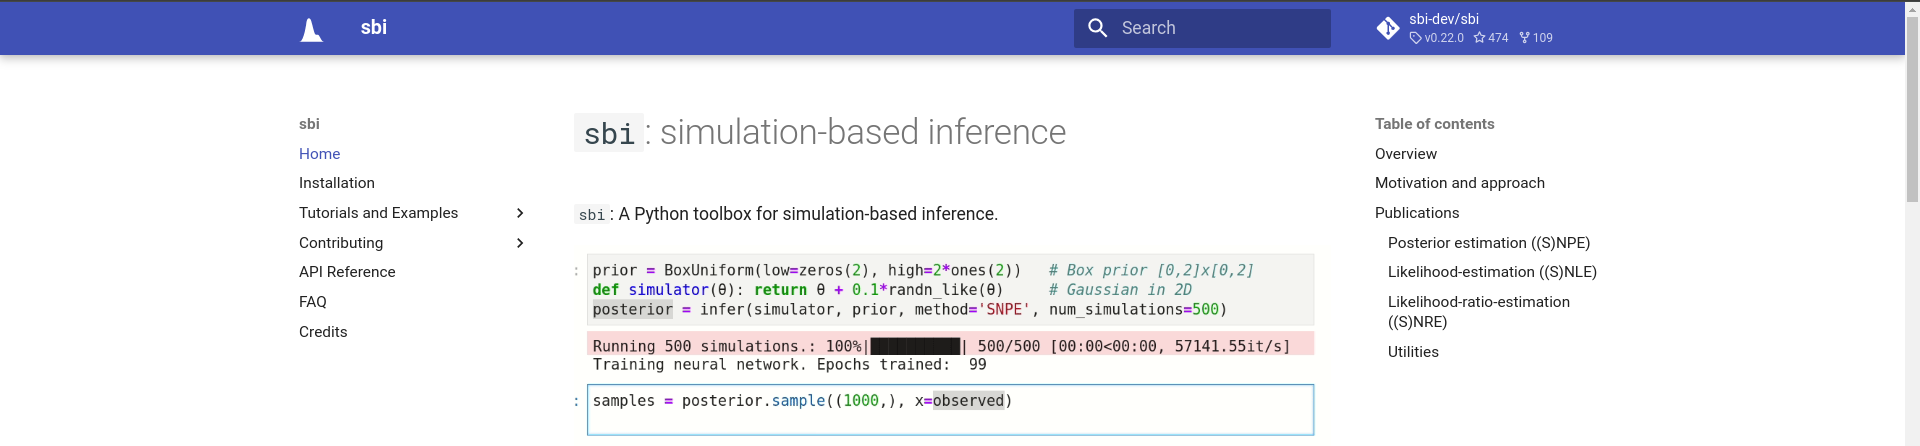
\includegraphics[width=\textwidth]{figures/sbi_screenshot}
        \href{https://github.com/sbi-dev}{github.com/sbi-dev}
        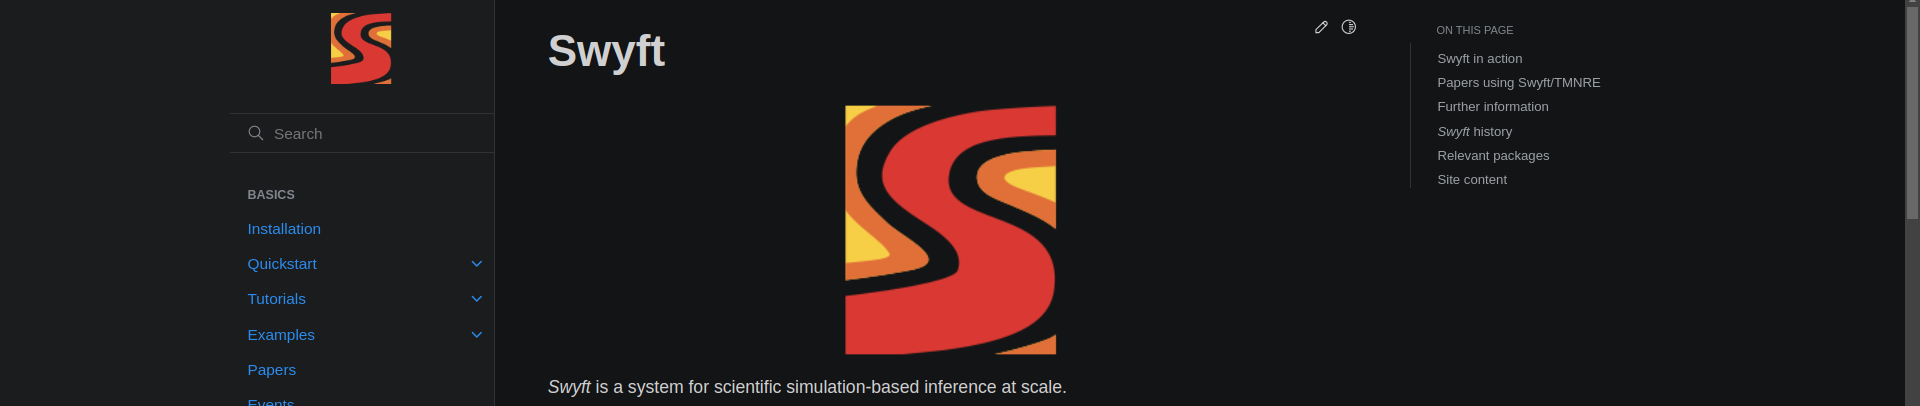
\includegraphics[width=\textwidth]{figures/swyft_screenshot}
        \href{https://github.com/undark-lab/swyft}{github.com/undark-lab/swyft}
        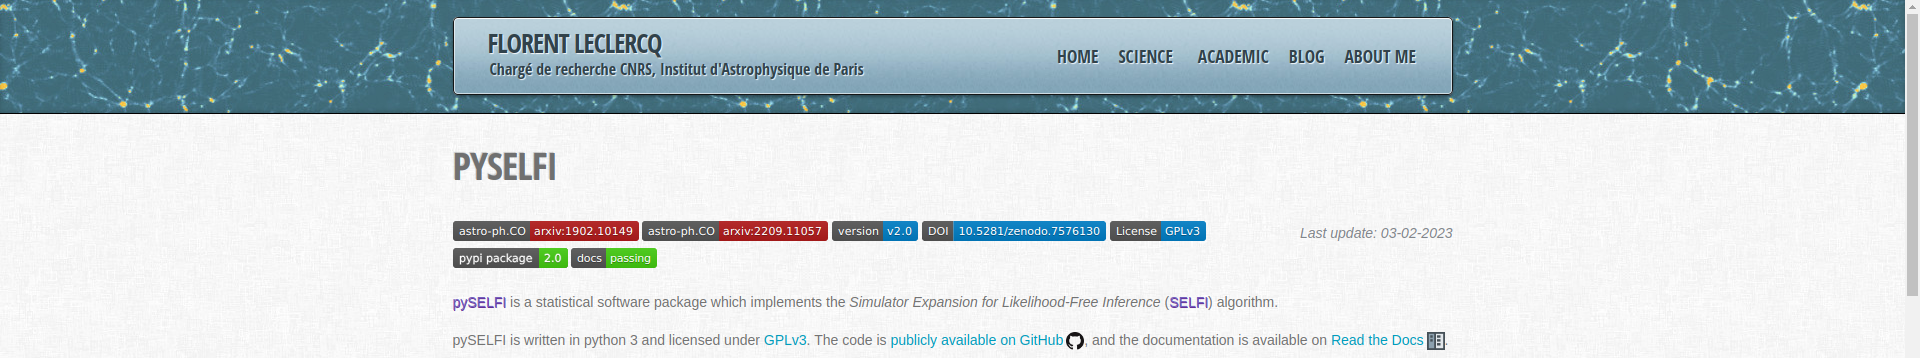
\includegraphics[width=\textwidth]{figures/selfi_screenshot}
        \href{https://github.com/florent-leclercq/pyselfi}{github.com/florent-leclercq/pyselfi}
        
\includegraphics[width=\textwidth]{figures/delfi_screenshot}
        \href{https://github.com/justinalsing/pydelfi}{github.com/justinalsing/pydelfi}
        


    \end{columns}
\end{frame}


\begin{frame}
    \frametitle{SBI \& model comparison}
    \begin{columns}
        \column{0.3\textwidth}
        \begin{itemize}
            \item Extend: models $A$ and $B$.
            \item Each with own separate parameters $\theta_A$ and $\theta_B$ (can be same).
            \item The evidence $\C[3]{\mathcal{Z}}(D|M)$ compares models
            \item Occams razor: more~predictive $\equiv$~more~probable \\(due to normalisation).
        \end{itemize}
        
        \column{0.7\textwidth}
        \includegraphics<1>[page=1, width=\textwidth]{figures/sbi_model_comparison.pdf}%
        \includegraphics<2>[page=2, width=\textwidth]{figures/sbi_model_comparison.pdf}%
        \includegraphics<3>[page=3, width=\textwidth]{figures/sbi_model_comparison.pdf}%
    \end{columns}
\end{frame}

\begin{frame}
    \frametitle{Nested sampling and Simulation based inference}
    \student{kilian_scheutwinkel}{Kilian Scheutwinkel}{PhD}
    \begin{columns}[t]
        \column{0.45\textwidth}
        \begin{block}{Weak SBI}
            \begin{itemize}
                \item Use model comparison to choose between likelihoods
                \item Use flexible likelihood (e.g. unknown noise scale $\sigma$, non-gaussian shape, mixture components~\arxiv{1809.04598})
                \item 21cm~\arxiv{2204.04491}, SNe~\arxiv{2312.02075}
            \end{itemize}

        \end{block}
        \column{0.45\textwidth}
        \begin{block}{Strong SBI}
            \begin{itemize}
                \item Develop ``likelihood-free nested sampling''
                \item Use dead points to train NRE
                \item Replaces/enhances current SotA of truncation techniques
            \end{itemize}
        \end{block}
    \end{columns}
    \centerline{
        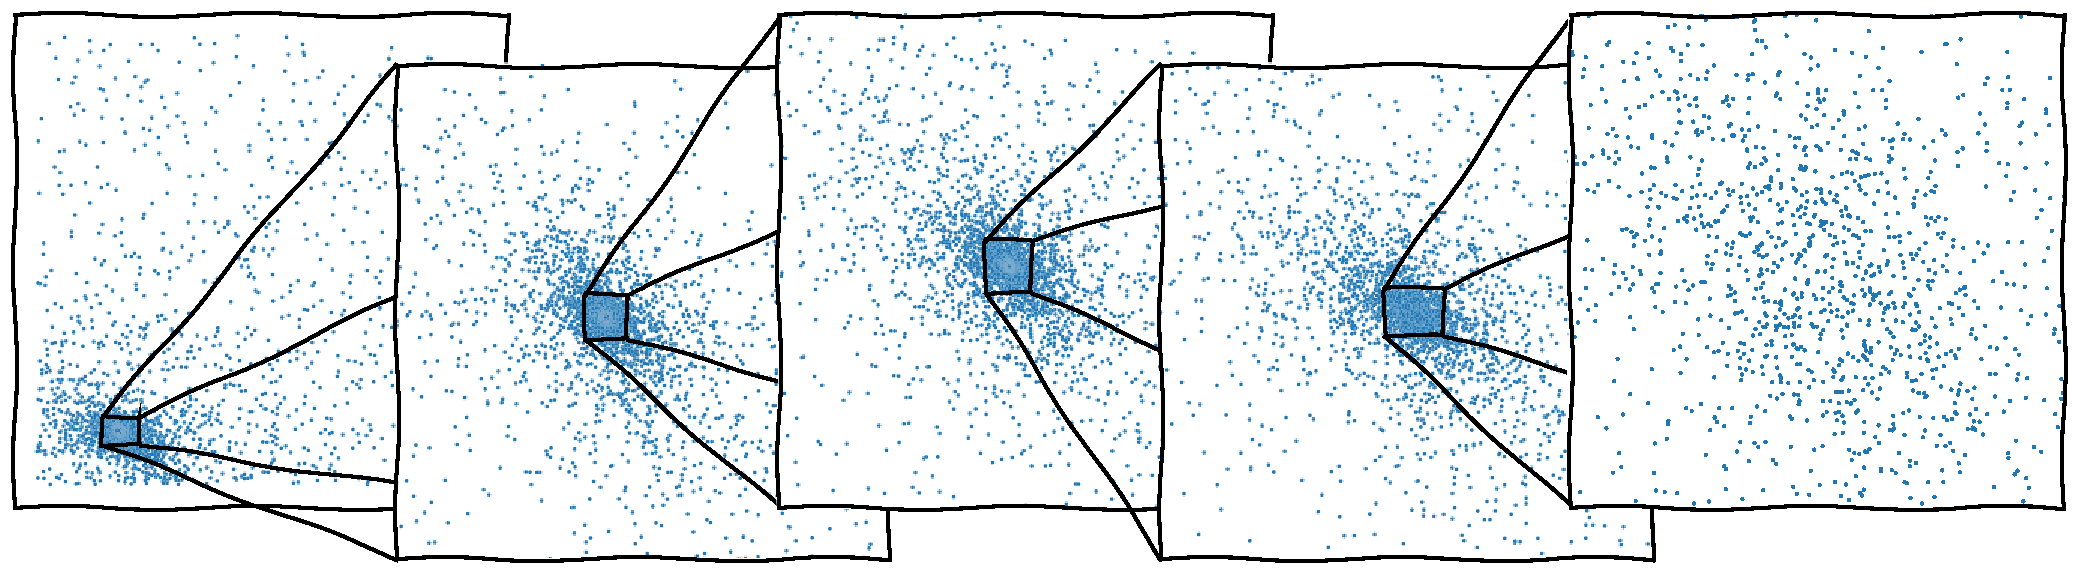
\includegraphics[width=0.8\textwidth]{figures/dead_measure}
    }
\end{frame}



\begin{frame}
    \frametitle{Cosmological forecasting}
    \framesubtitle{Have you ever done a Fisher forecast, and then felt Bayesian guilt?}
    \vspace{-20pt}
    \begin{columns}[t]
        \column{0.5\textwidth}
        \begin{itemize}
            \item Cosmologists are interested in forecasting what a Bayesian analysis of future data might produce.
            \item Useful for:
                \begin{itemize}
                    \item white papers/grants,
                    \item optimising existing instruments/strategies,
                    \item picking theory/observation to explore next.
                \end{itemize}
            \item To do this properly:
                \begin{enumerate}
                    \item start from current knowledge $\pi(\theta)$, derived from current data
                    \item Pick potential dataset $D$ that might be collected from $P(D)\: (=\mathcal{Z})$
                    \item Derive posterior $P(\theta|D)$
                    \item Summarise science (e.g. constraint on $\theta$, ability to perform model comparison)
                \end{enumerate}
        \end{itemize}

        \column{0.5\textwidth}
        \begin{itemize}
            \item This procedure should be marginalised over:
                \begin{enumerate}
                    \item All possible parameters $\theta$ (consistent with prior knowledge)
                    \item All possible data $D$
                \end{enumerate}
            \item i.e. marginalised over the joint $P(\theta,D)=P(D|\theta)P(\theta)$.
            \item Historically this has proven very challenging.
            \item Most analyses assume a fiducial cosmology $\theta_*$, and/or a Gaussian likelihood/posterior (c.f. Fisher forecasting).
            \item This runs the risk of biasing forecasts by baking in a given theory/data realisation.
        \end{itemize}
        
    \end{columns}

\end{frame}

\begin{frame}
    \frametitle{Fully Bayesian Forecasting~\arxiv{2309.06942}}
    \student{thomas_gessey-jones}{Thomas Gessey-Jones}{PhD}
    \begin{columns}
        \column{0.5\textwidth}
        \begin{itemize}
            \item Simulation based inference gives us the language to marginalise over parameters $\theta$ and possible future data $D$.
            \item Evidence networks give us the ability to do this at scale for forecasting.
            \item Demonstrated in 21cm global experiments, marginalising over:
                \begin{itemize}
                    \item theoretical uncertainty
                    \item foreground uncertainty
                    \item systematic uncertainty
                \end{itemize}
            \item Able to say ``at 67mK radiometer noise'', have a 50\% chance of 5$\sigma$ Bayes factor detection.
            \item Can use to optimise instrument design
            \item Re-usable package: \texttt{prescience}
        \end{itemize}
        \column{0.5\textwidth}
        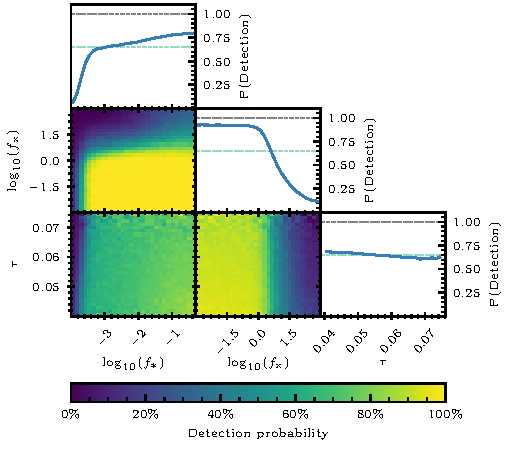
\includegraphics[width=\textwidth]{figures/fbf.pdf}
    \end{columns}
\end{frame}



\begin{frame}
    \frametitle{Conclusions}
    \framesubtitle{\href{https://www.github.com/handley-lab}{github.com/handley-lab}}
    \tikz[overlay,remember picture]
        \node[anchor=north east] (A) at ($(current page.north east)+(0,0)$) {
            
\includegraphics[width=0.09\textheight]{figures/students/adam_ormondroyd.jpg}%
            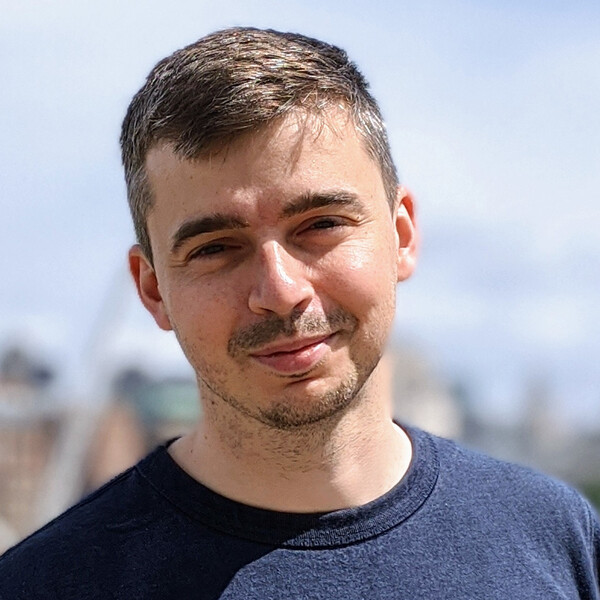
\includegraphics[width=0.09\textheight]{figures/students/david_yallup.jpg}%
            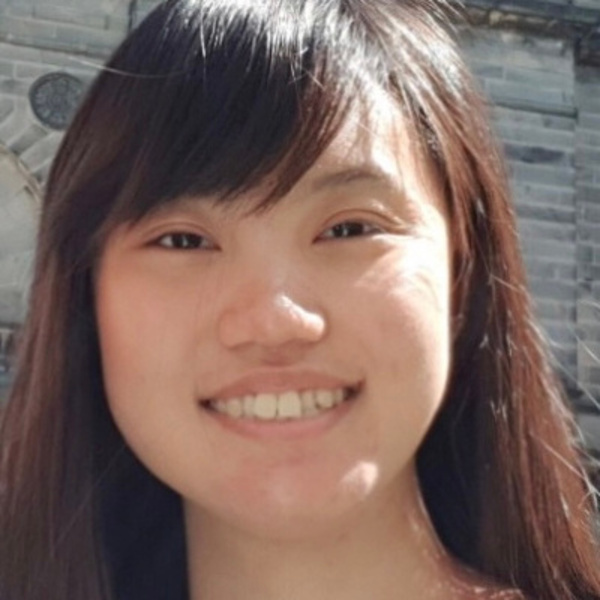
\includegraphics[width=0.09\textheight]{figures/students/dily_ong.jpg}%
            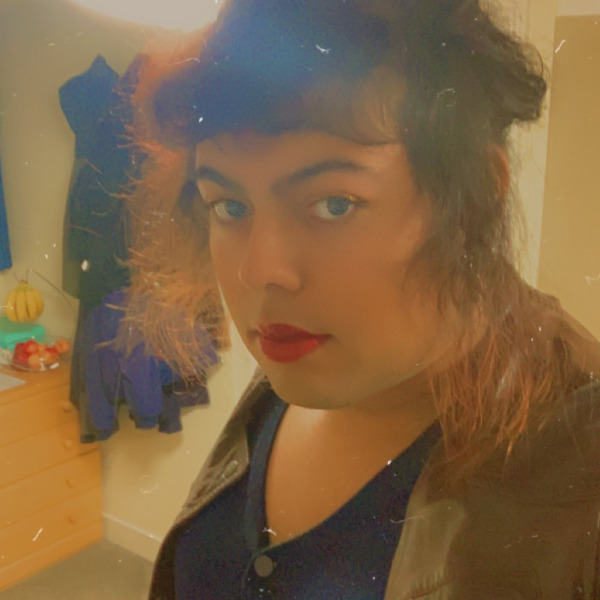
\includegraphics[width=0.09\textheight]{figures/students/felicity_ibrahim.jpg}%
            
\includegraphics[width=0.09\textheight]{figures/students/george_carter.jpg}%
            \includegraphics[width=0.09\textheight]{figures/students/harry_bevins.jpg}%
            \includegraphics[width=0.09\textheight]{figures/students/ian_roque.jpg}%
            \includegraphics[width=0.09\textheight]{figures/students/kilian_scheutwinkel.jpg}%
            \includegraphics[width=0.09\textheight]{figures/students/metha_prathaban.jpg}%
            \includegraphics[width=0.09\textheight]{figures/students/namu_kroupa.jpg}%
            \includegraphics[width=0.09\textheight]{figures/students/sinah_legner.jpg}%
            \includegraphics[width=0.09\textheight]{figures/students/thomas_gessey-jones.jpg}%
            \includegraphics[width=0.09\textheight]{figures/students/tze_goh.jpg}%
            \includegraphics[width=0.09\textheight]{figures/students/wei-ning_deng.jpg}%
    };
    Covered a suite of tools for next-generation ``generative cosmology''
    \begin{itemize}
        \item Nested sampling for cosmological\ldots
            \begin{itemize}
                \item model comparison
                \item parameter estimation
                \item tension quantification
            \end{itemize}
        \item Nuisance-marginalised cosmology
            \boxed{
                \C[2]{\mathcal{L}}(\theta) 
                = 
                \frac{
                    \C[0]{\mathcal{P}}(\theta)
                    \C[3]{\mathcal{Z}}
                }{
                    \C[1]{\pi}(\theta)
                }
            }
        \item Simulation-based inference
        \item Fully Bayesian forecasting
    \end{itemize}
\end{frame}

\end{document}
